%!TEX root = ../template.tex
%%%%%%%%%%%%%%%%%%%%%%%%%%%%%%%%%%%%%%%%%%%%%%%%%%%%%%%%%%%%%%%%%%%%
%% chapter2.tex
%% NOVA thesis document file
%%
%% Chapter 2: State of the Art
%%%%%%%%%%%%%%%%%%%%%%%%%%%%%%%%%%%%%%%%%%%%%%%%%%%%%%%%%%%%%%%%%%%%

\typeout{NT FILE chapter2.tex}%

\chapter{State of the Art}
\label{cha:stateoftheart}

\prependtographicspath{{5-Figures/Covers/}}

\epigraphfontsize{\small\itshape}
\setlength\epigraphwidth{12.5cm}
\setlength\epigraphrule{0pt}

This chapter presents the background, standards, and related work for this dissertation. It reviews the main technologies behind smart manufacturing, digital twins, asset administration shells, and simulation environments, identifying the key gaps this work addresses.

The chapter is organized into six sections:
\begin{itemize}
    \item \Cref{sec:i40_evolution} describes the evolution of manufacturing systems, the main enabling technologies, and the \gls{RAMI} reference architecture.
    \item \Cref{sec:dt_paradigm} explains the \gls{DT} concept, its history, data flow classifications, lifecycle stages, and general architectures.
    \item \Cref{sec:semantic_interoperability} focuses on semantic modeling using the \gls{AAS} (\gls{IEC}~63278), submodel templates from the \gls{IDTA}, the \gls{AASX} package format, and open-source tools.
    \item \Cref{sec:game_engines_vc} discusses the use of game engines in industrial automation, CAD conversion challenges, kinematic simulation, and network communication.
    \item \Cref{sec:automated_dt_generation} reviews existing methods for generating digital twins automatically, grouping them into model-driven, data-driven, and AI-based methods.
    \item \Cref{sec:sota_gaps} discusses current limitations in the literature and outlines the research opportunities addressed by this dissertation.
\end{itemize}

%=============================================================================
\section{Evolution of Production Systems in Industry 4.0}
\label{sec:i40_evolution}
%=============================================================================

Manufacturing systems have evolved through several stages, from early mechanization to modern automated and networked factories \cite{Hermann2016,Kagermann2022}. The fourth industrial revolution, or Industry 4.0 \cite{Kagermann2022}, connects physical shop-floor machinery with digital systems, forming what are known as \glspl{CPPS}.

\subsection{Manufacturing Paradigms: From Dedicated to Reconfigurable Systems}

In the 20th century, factories mostly relied on \glspl{DMS}. These systems used fixed production lines to produce large volumes of identical products at low cost. However, they were difficult and expensive to change when product designs evolved \cite{Khan2025,Rocha2024}.

To handle wider product varieties, \glspl{FMS} were developed, using automated handling and \glspl{CNC} to produce pre-defined part families. Later, \glspl{RMS} were introduced to allow faster and cheaper changes. An \gls{RMS} is designed to be modular, integrable, customizable, scalable, convertible, and diagnosable \cite{Khan2025}. In an \gls{RMS}, machines, conveyors, and workstations can be added, removed, or rearranged as needed. To support this level of flexibility without long downtimes, software systems must be able to discover, configure, and connect new equipment automatically, without manual reprogramming of simulation scenes or controller software \cite{Rocha2024,Ahvanouee2025}.

\Cref{fig:industry_evolution} shows the progression across the four industrial revolutions, moving from steam-powered machines to modern networked systems.

\begin{figure}[htbp]
    \centering
    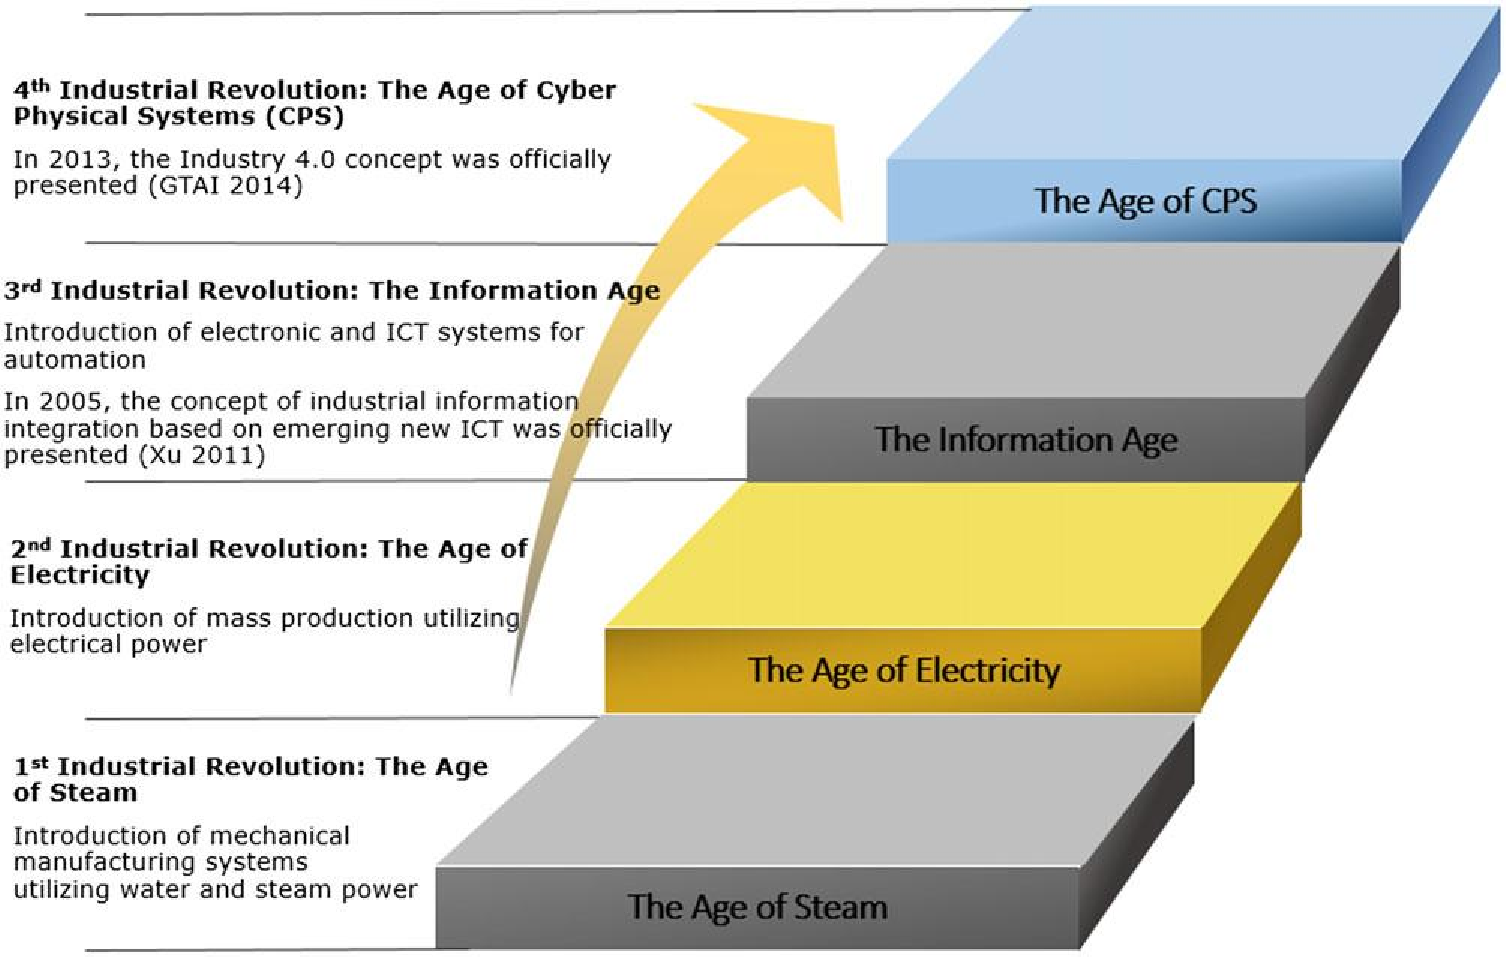
\includegraphics[width=0.88\textwidth]{5-Figures/i4.0_history.pdf} 
    \caption{Evolution from Industry 1.0 to Industry 4.0 \cite{Xu2018}.}
    \label{fig:industry_evolution}
\end{figure}

\subsection{Enabling Technologies of Smart Manufacturing}

Several core technologies work together to make \glspl{CPPS} possible:
\begin{itemize}
    \item \textbf{\glspl{CPS} and \glspl{CPPS}:} Connect physical machinery with sensors, microcontrollers, and communication networks \cite{Abdel-Aty2022}, allowing devices to coordinate actions and collect real-time data \cite{AshtariTalkhestani2019}.
    \item \textbf{\gls{IIOT} and Edge Computing:} Provides reliable networking between shop-floor devices and controllers. Processing data near the machines reduces network load and communication delays \cite{Amthiou2023,Jones2020}.
    \item \textbf{Cloud Computing and \gls{MAAS}:} Enables storage and heavy computing tasks in the cloud, helping companies share production resources and run plant-wide optimization algorithms \cite{Xu2018,Amthiou2023}.
    \item \textbf{Semantic Interoperability and Information Modeling:} Uses standardized data models so that different software tools can share mechanical, electrical, and operational machine data without translation errors \cite{Drath2008,Lu2025}.
    \item \textbf{The \gls{DT}:} Serves as a digital representation of a physical asset, combining real-time sensor data, 3D visualization, and simulation models \cite{Tao2019,Jones2020}.
\end{itemize}

\subsection{Reference Architectural Model Industrie 4.0 (RAMI 4.0)}
\label{sec:rami}

Because Industry 4.0 involves many different standards and vendors, Plattform Industrie 4.0 defined \gls{RAMI} (\gls{DIN} \gls{EN} \gls{IEC}~63088). \gls{RAMI} provides a common three-dimensional model to organize industrial assets across their entire lifecycle, factory hierarchy, and software layers \cite{Pajpach2025}, as shown in \Cref{fig:rami40_structure}.

\begin{figure}[htbp]
    \centering
    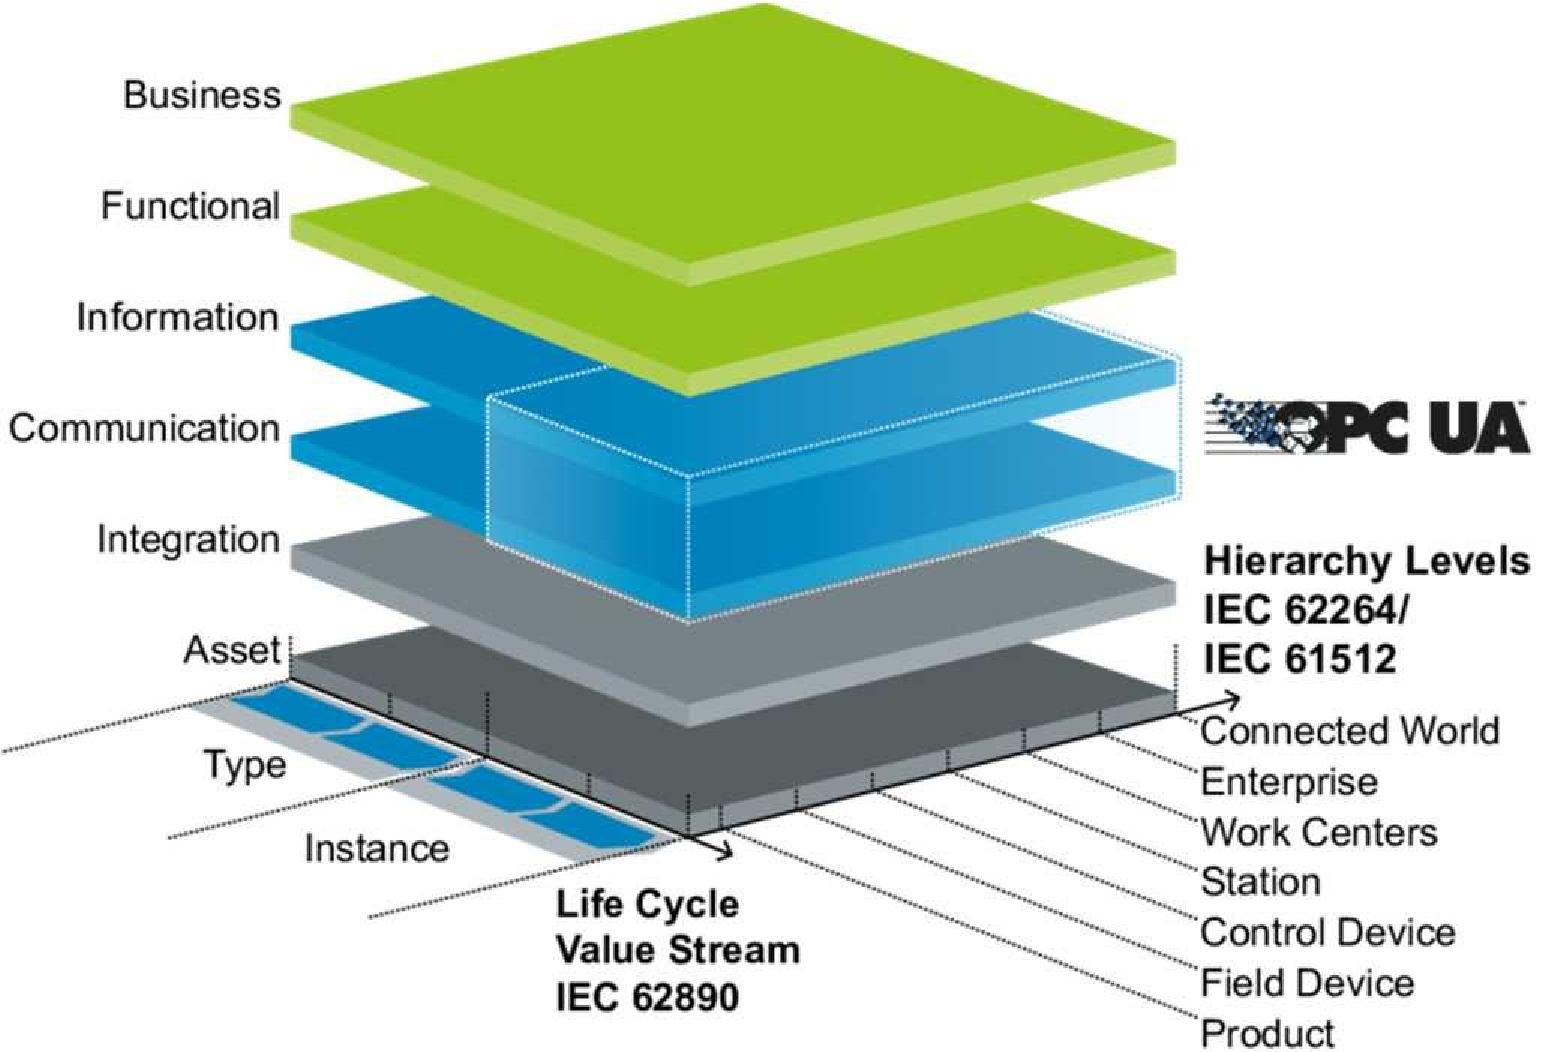
\includegraphics[width=0.88\textwidth]{5-Figures/rami.pdf}
    \caption{The three-dimensional architecture of RAMI 4.0 \cite{Pajpach2025}.}
    \label{fig:rami40_structure}
\end{figure}

The three axes of \gls{RAMI} are defined as follows:
\begin{enumerate}
    \item \textbf{Layers (Vertical Axis):} Divides industrial systems into six viewpoints:
    \begin{itemize}
        \item \textit{Asset Layer:} The physical equipment, including machines, tools, cables, and operators.
        \item \textit{Integration Layer:} The boundary that connects physical hardware to computers using sensors, barcodes, and interfaces.
        \item \textit{Communication Layer:} Communication protocols and network connections, such as \gls{OPCUA}, \gls{MQTT}, and \gls{REST}.
        \item \textit{Information Layer:} Data models, parameters, and variable definitions.
        \item \textit{Functional Layer:} Control logic, application code, and simulation models.
        \item \textit{Business Layer:} Enterprise systems, production orders, and overall process rules.
    \end{itemize}
    
    \item \textbf{Life Cycle and Value Stream (Horizontal Axis):} Based on \gls{IEC}~62890, this axis separates the design phase (``Type'') from the operational phase (``Instance''), helping track an asset from initial engineering to decommissioning.
    
    \item \textbf{Hierarchy Levels (Third Axis):} Extends the standard automation levels (\gls{IEC}~62264 and \gls{IEC}~61512) to include: \textit{Product}, \textit{Field Device}, \textit{Control Device}, \textit{Station}, \textit{Work Centers}, \textit{Enterprise}, and \textit{Connected World}.
\end{enumerate}

In \gls{RAMI}, any asset that has a digital identity and connects to the network is called an \textit{Industry 4.0 Component}. It consists of the physical asset combined with its digital representation, called the \gls{AAS} \cite{Abdel-Aty2022,Pajpach2025}. The \gls{AAS} links the Asset and Integration layers, providing a standard way to access machine data and functions.

%=============================================================================
\section{The Digital Twin Paradigm in Manufacturing}
\label{sec:dt_paradigm}
%=============================================================================

In modern manufacturing, digital twins are widely used for monitoring, testing, and optimization. However, the term is often applied loosely to any 3D animation or simple dashboard \cite{Kritzinger2018}. A clear definition is needed to separate simple models from true digital twins.

\subsection{Historical Evolution of the Paradigm}
\label{subsec:dt_history}

The idea of using digital models to mirror real systems dates back to NASA's Apollo program, where ground simulators replicated spacecraft conditions during missions \cite{Khan2025}. The term ``Digital Twin'' was introduced in 2002 by Michael Grieves for product lifecycle management \cite{Grieves2014,Jones2020}.

In 2012, NASA and the U.S. Air Force defined the digital twin as an integrated multi-physics simulation of a vehicle or system that uses sensor data and operational history to mirror the life of its physical twin \cite{Shafto2012}. As shown in \Cref{fig:dt_timeline}, \textcite{Khan2025} divide this evolution into three periods:
\begin{itemize}
    \item \textbf{Theorization (1970 to 2010):} Early concepts developed mainly in aerospace, using isolated offline simulation models without real-time shop-floor connections.
    \item \textbf{Consolidation (2010 to 2016):} The concept expanded to manufacturing and automation, driven by Industry 4.0, lower sensor costs, and predictive maintenance.
    \item \textbf{Expansion and Standardization (2016 to Present):} Widespread use of open standards such as \gls{AAS}, \gls{OPCUA}, and \gls{FMI}, alongside real-time game engines for interactive simulation \cite{Khan2025,Gil2024}.
\end{itemize}

\begin{figure}[htbp]
    \centering
    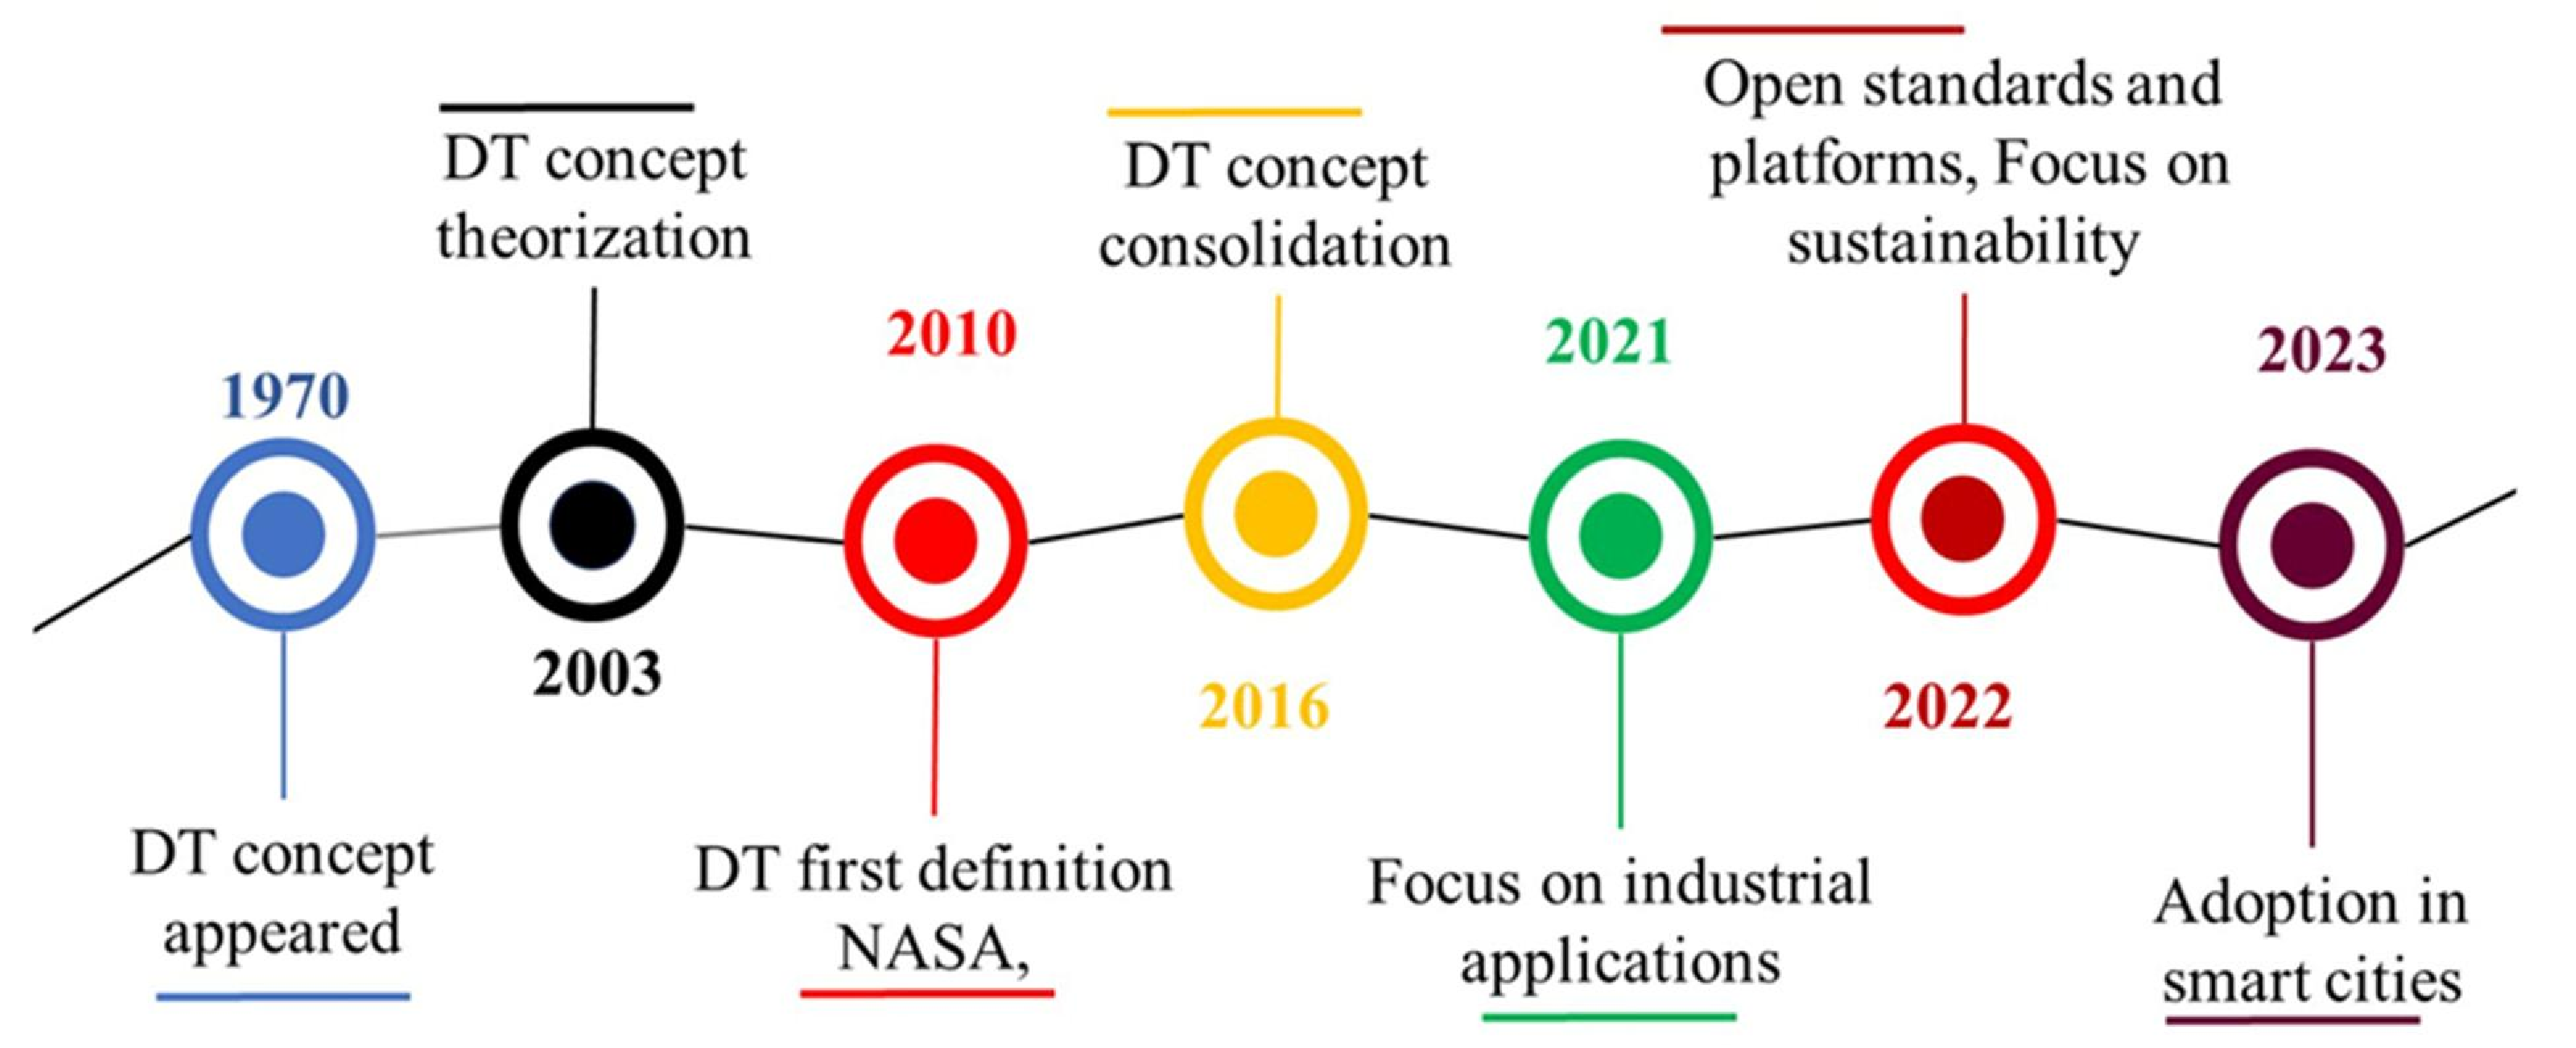
\includegraphics[width=0.88\textwidth]{5-Figures/dt_timeline.pdf}
    \caption{Timeline of Digital Twin evolution across industrial eras \cite{Khan2025}.}
    \label{fig:dt_timeline}
\end{figure}

\subsection{Taxonomy of Virtual Representations: DM, DS, and DT}
\label{subsec:dt_definition}

To clarify what constitutes a digital twin, this dissertation follows the classification from \textcite{Kritzinger2018}, which separates virtual representations by the level of automated data flow between the physical and digital systems.

\subsubsection{Digital Model (DM)}

A \gls{DM} has manual data exchange in both directions (\Cref{fig:taxonomy_dm}). Static \gls{CAD} drawings, offline kinematic studies, and spreadsheets are typical examples. If changes are made to the physical machine, an engineer must manually update the software model. Likewise, changes made in the model must be implemented by hand on the shop floor.

\subsubsection{Digital Shadow (DS)}

A \gls{DS} has automated, one-way data flow from the physical asset to the digital model (\Cref{fig:taxonomy_ds}). Sensors and controller tags send live data to the virtual model, so the digital representation updates automatically when the machine moves or changes state. However, the data flow is one-way: the digital shadow does not send control commands back to the machine.

\subsubsection{Digital Twin (DT)}

A \gls{DT} has automated, two-way data flow between the physical asset and the digital representation (\Cref{fig:taxonomy_dt}). Sensor readings and controller states update the virtual model automatically, while simulations or decisions made in the digital environment can send commands back to the physical controller to change its operation.

\begin{figure}[htbp]
    \centering
    \begin{subfigure}[b]{0.32\textwidth}
        \centering
        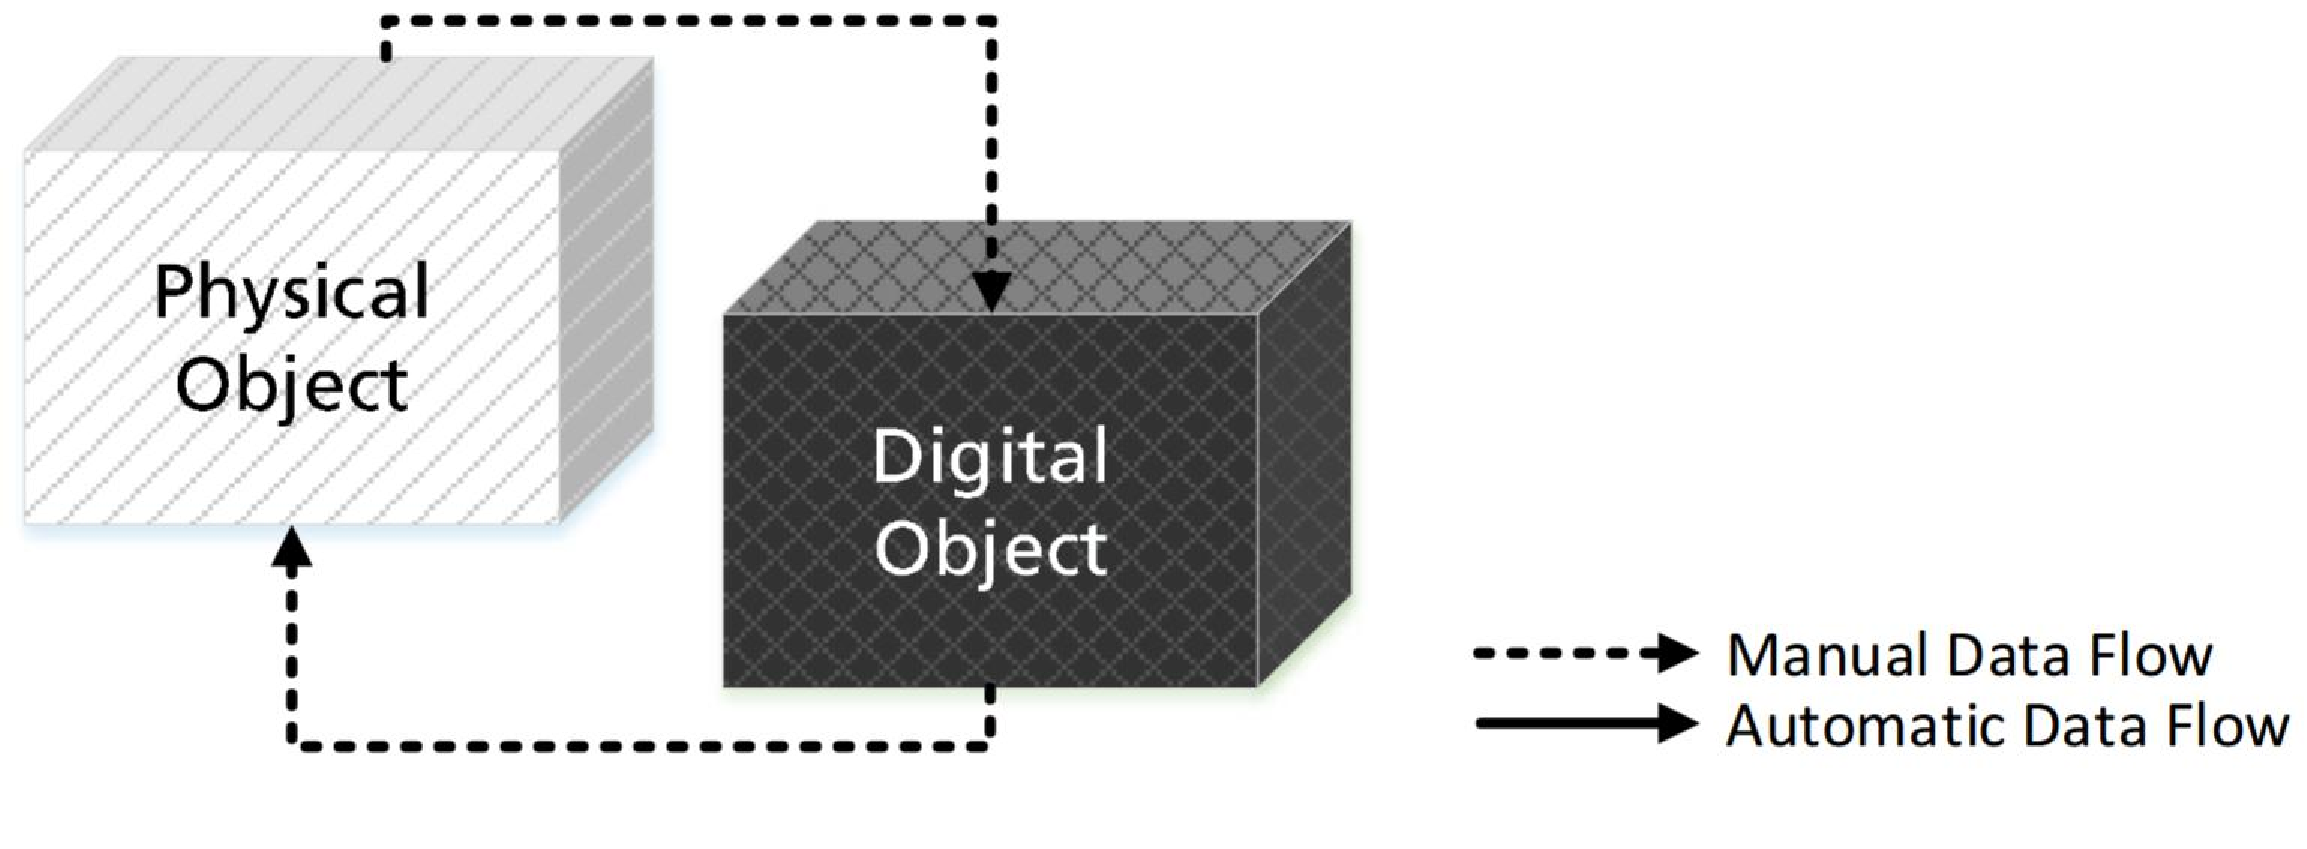
\includegraphics[width=\textwidth]{5-Figures/digital_model_flow.pdf}
        \caption{Digital Model (DM).}
        \label{fig:taxonomy_dm}
    \end{subfigure}
    \hfill
    \begin{subfigure}[b]{0.32\textwidth}
        \centering
        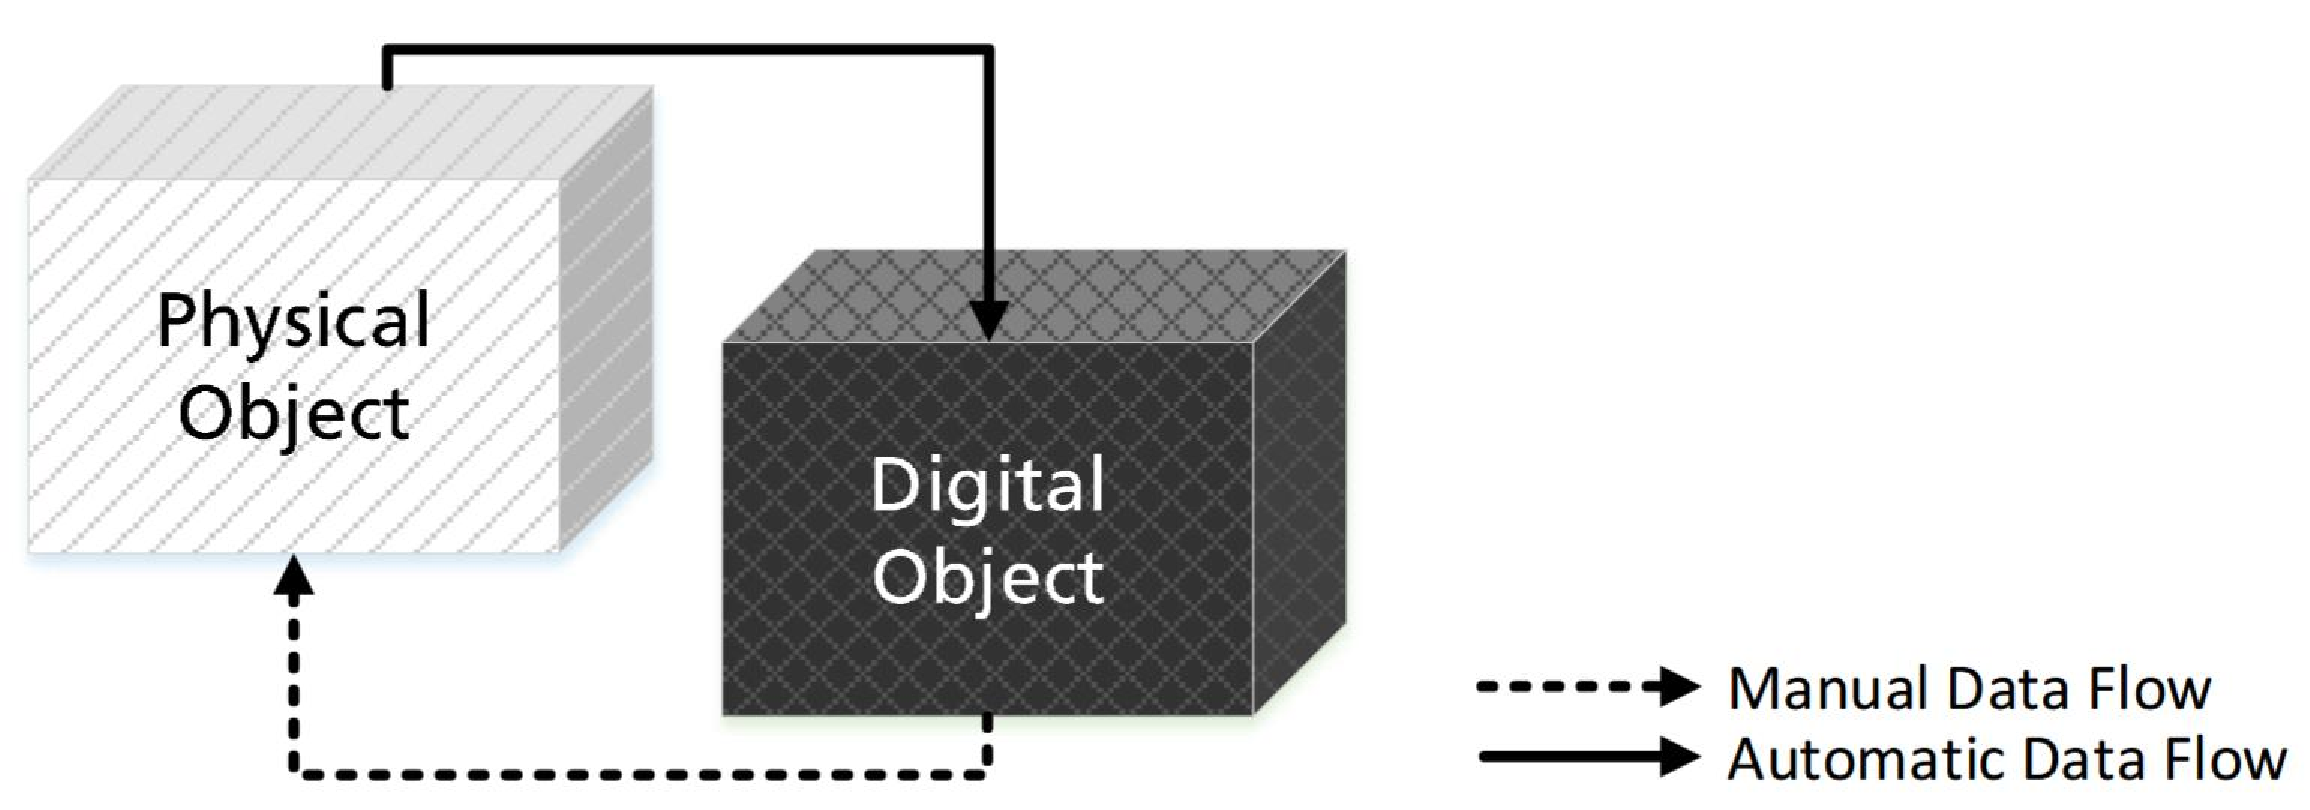
\includegraphics[width=\textwidth]{5-Figures/digital_shadow_flow.pdf}
        \caption{Digital Shadow (DS).}
        \label{fig:taxonomy_ds}
    \end{subfigure}
    \hfill
    \begin{subfigure}[b]{0.32\textwidth}
        \centering
        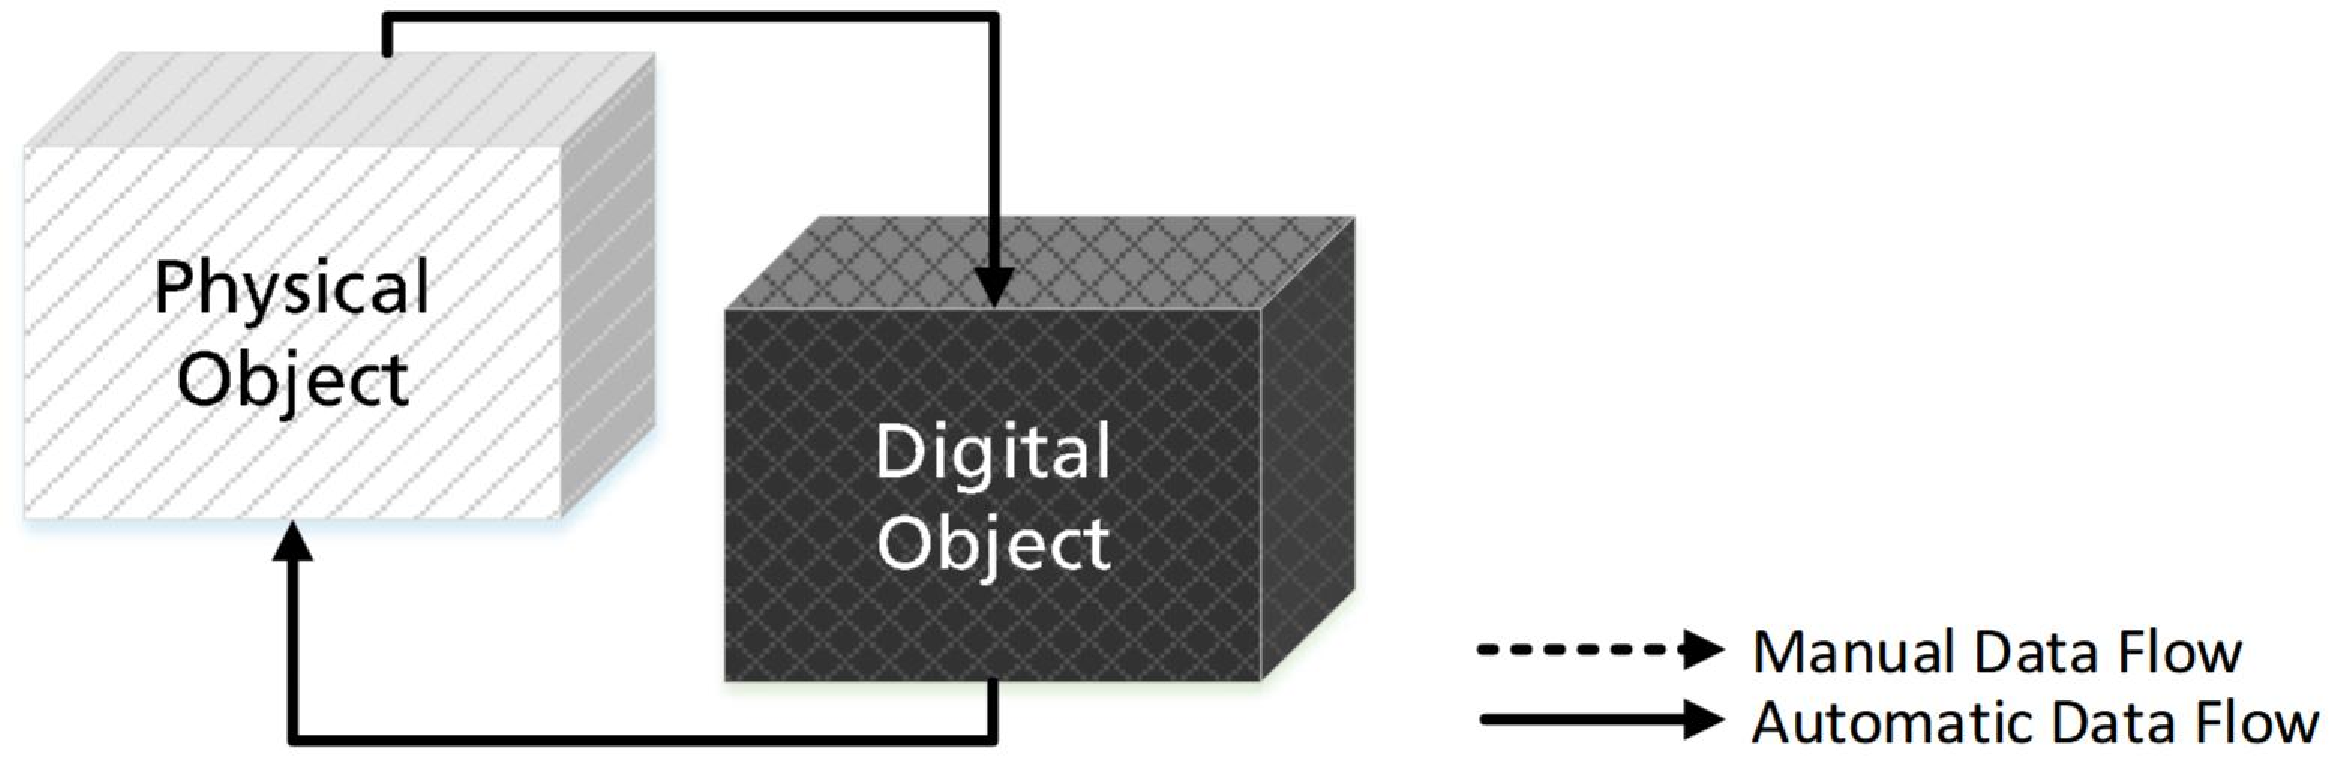
\includegraphics[width=\textwidth]{5-Figures/digital_twin_flow.pdf}
        \caption{Digital Twin (DT).}
        \label{fig:taxonomy_dt}
    \end{subfigure}
    \caption{Taxonomy of virtual representations classified by automated data flow: (a) Digital Model, (b) Digital Shadow, and (c) Digital Twin \cite{Kritzinger2018}.}
    \label{fig:dt_taxonomy_comparison}
\end{figure}

Under this definition, many commercial systems sold as digital twins are actually digital shadows, since they only display live data and cannot control the equipment. The framework proposed in this dissertation is designed for full \gls{DT} capability, supporting both live two-way synchronization and offline virtual commissioning.

\subsection{The Digital Twin Lifecycle}

A digital twin evolves with the machine over its lifecycle \cite{Jones2020,Khan2025}, passing through five main phases:
\begin{enumerate}
    \item \textbf{Design and Modeling:} Starts as a \gls{DM} during early engineering, where CAD shapes and expected kinematics are tested before building the machine.
    \item \textbf{Virtual Commissioning:} Tests controller programs against the virtual model before physical installation, using software emulation or physical PLCs to catch logic errors early \cite{Striffler2023}.
    \item \textbf{Operational Connectivity:} The machine is installed and connected to the digital twin, establishing live data links to mirror actual movements and states.
    \item \textbf{Optimization and Control:} Operating data is used to improve performance, detect faults, and adjust setpoints on the physical machine \cite{Tao2019}.
    \item \textbf{Reconfiguration and Decommissioning:} When lines are reorganized or parts replaced, the digital twin updates its structure to match the new physical setup.
\end{enumerate}

\subsection{Reference Architectures for Industrial Digital Twins}

Several reference architectures have been proposed for digital twins \cite{Semeraro2021}. \textcite{Tao2019} describe a five-part model: physical entity, virtual entity, services, data, and connection links. \textcite{AshtariTalkhestani2019} present an intelligent architecture that adds software agents for plug-and-produce operations.

In line with these concepts, this dissertation uses a four-layer architecture:
\begin{itemize}
    \item \textbf{Physical Layer:} Machinery, conveyors, sensors, and \glspl{PLC} on the shop floor.
    \item \textbf{Authoring Layer:} Tools used to convert 3D CAD files into lightweight models and attach operational properties.
    \item \textbf{Middleware and Registry Layer:} Servers such as Eclipse BaSyx that store and share standardized \gls{AAS} data over network \glspl{API}.
    \item \textbf{Simulation and Runtime Layer:} A 3D game engine (Unity) that builds the virtual scene, runs physics, and connects with controllers.
\end{itemize}

%=============================================================================
\section{Semantic Modeling and Interoperability Standards}
\label{sec:semantic_interoperability}
%=============================================================================

Building digital twins automatically requires standard, machine-readable formats. Without standard descriptions for geometry, kinematics, electrical pins, and logic rules, each tool requires custom translation scripts \cite{Ahvanouee2025,Barnard2024}.

Earlier efforts often used \gls{AML} (\gls{IEC}~62714) to share plant structure and 3D files during the engineering phase \cite{Drath2008}. However, \gls{AML} was designed as an offline file format for project handover. It does not provide network \glspl{API} or standard servers for live shop-floor communication \cite{Barnard2024,Ahvanouee2025}.

To provide a standard digital wrapper that works during both design and runtime, Plattform Industrie 4.0 created the \gls{AAS} (\gls{IEC}~63278) \cite{Pajpach2025,Abdel-Aty2022}.

\subsection{Asset Administration Shell Architecture and Metamodel}
\label{subsec:aas_deep_dive}

The \gls{AAS} serves as the digital representation of an industrial asset, containing its identification, technical data, and software interfaces \cite{Abdel-Aty2022,Pajpach2025}, as shown in \Cref{fig:aas_introduction}.

\begin{figure}[htbp]
    \centering
    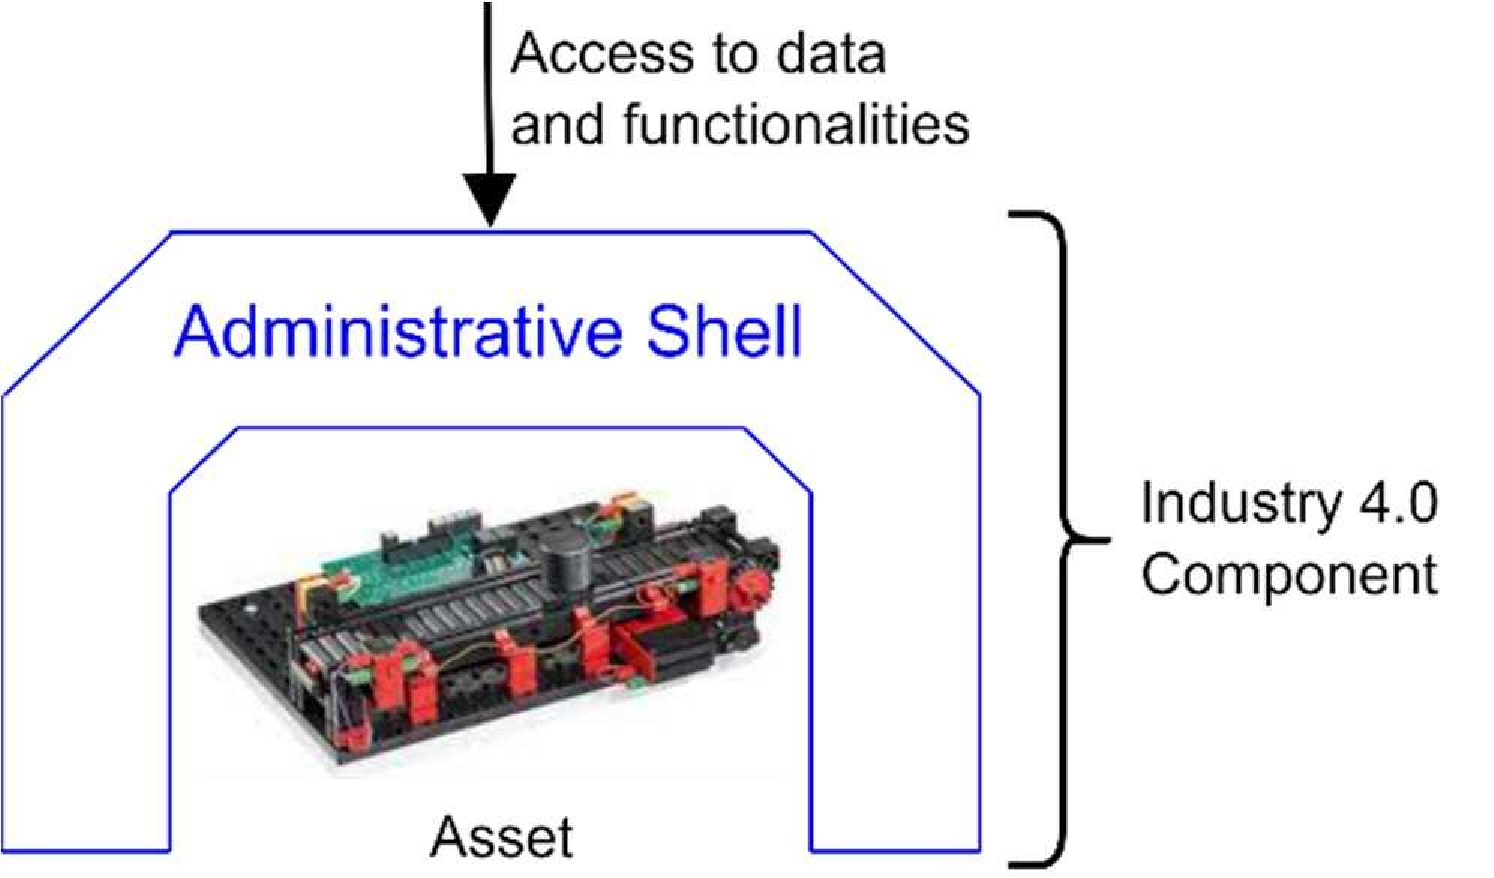
\includegraphics[width=0.85\textwidth]{5-Figures/AAS_introduction.pdf} 
    \caption{Industry 4.0 Component and Asset Administration Shell structure \cite{Pajpach2025}.}
    \label{fig:aas_introduction}
\end{figure}

The \gls{AAS} metamodel, defined by the \gls{IDTA}, includes the following key parts:
\begin{itemize}
    \item \textbf{\gls{AAS} Container:} The top-level container, identified by a unique ID (\gls{URI} or \gls{UUID}).
    \item \textbf{Asset Information:} States whether the asset is a generic product type or a specific physical unit on the shop floor.
    \item \textbf{Submodel:} A group of related properties for a specific domain, such as identification, technical specs, or kinematics. Each submodel has an identifier and a reference to a standardized semantic definition (such as \gls{ECLASS} or IDTA templates).
    \item \textbf{Submodel Elements:} The actual data fields within a submodel:
    \begin{itemize}
        \item \texttt{Property}: Stores a single value, such as a number, text, or boolean.
        \item \texttt{MultiLanguageProperty}: Stores text in multiple languages.
        \item \texttt{Range}: Sets minimum and maximum limits for a numerical value.
        \item \texttt{File} and \texttt{Blob}: References or embeds files, such as 3D meshes, user manuals, or drawings.
        \item \texttt{SubmodelElementCollection} and \texttt{SubmodelElementList}: Groups multiple submodel elements together.
        \item \texttt{Operation}: Defines invokable functions with input and output parameters.
    \end{itemize}
\end{itemize}

\subsection{Standardized Submodel Templates and IDTA Specifications}

The main benefit of the \gls{AAS} is that different systems can read data without custom code if they follow standardized \textit{Submodel Templates} from the \gls{IDTA}. Common templates include:
\begin{itemize}
    \item \textbf{Digital Nameplate (IEC 61406):} Replaces physical nameplates with machine-readable serial numbers, manufacturer details, and conformity marks.
    \item \textbf{Technical Data:} Holds operating limits, dimensions, voltages, and power ratings.
    \item \textbf{Contact Information:} Lists manufacturer contact details for maintenance and support.
\end{itemize}

While these templates cover general information, templates for real-time physics, kinematics, and control logic are still emerging in the literature \cite{Pajpach2025,Perez2025}. This is one of the main areas where this dissertation defines and tests custom submodel structures.

\subsection{Portable Packaging: The AASX Container}

To make it easy to share digital twin assets across different computers and tools, the standard defines the \gls{AASX} package (\gls{IEC}~63278-1). The \gls{AASX} format uses the Open Packaging Convention (\gls{OPC}), the same container format used by common office documents.

An \gls{AASX} package bundles:
\begin{enumerate}
    \item The \gls{AAS} and its submodels saved as \gls{JSON} or \gls{XML}.
    \item Embedded binary files, such as 3D meshes (\gls{GLB}/\gls{glTF}), wiring diagrams, and icons.
    \item Relationship files that link the data together.
\end{enumerate}

Using \gls{AASX} allows an asset to be distributed as a single file. An application can download the package and immediately load its 3D model, joints, pin mappings, and connection addresses without needing extra files.

\Cref{fig:pajpach_aasx_conveyor} illustrates how a physical conveyor module is traditionally modeled inside the standard \gls{IDTA} toolchain using the official AASX Package Explorer \cite{Pajpach2025}. In conventional workflows, the automation engineer must manually populate extensive hierarchical tables, defining properties, ranges, and submodel element collections without visual feedback or spatial awareness of the physical asset.

\begin{figure}[htbp]
    \centering
    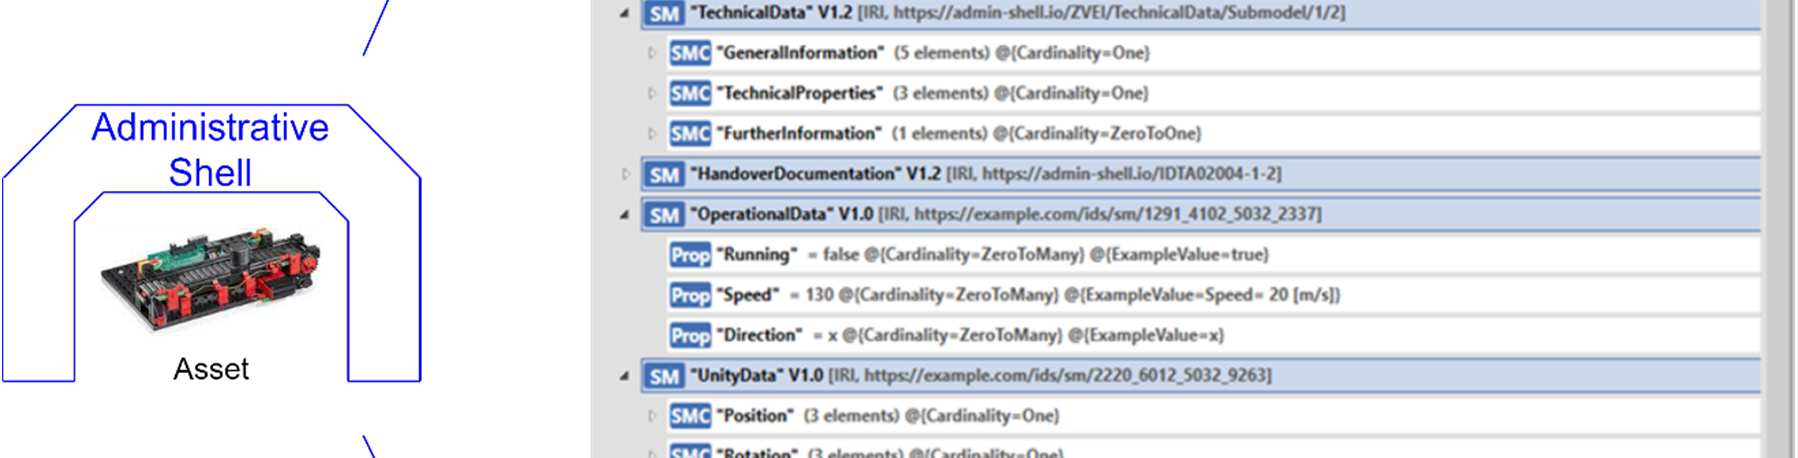
\includegraphics[width=0.92\textwidth]{5-Figures/pajpach_aasx_conveyor}
    \caption{Digital description of a modular conveyor within the official AASX Package Explorer \cite{Pajpach2025}.}
    \label{fig:pajpach_aasx_conveyor}
\end{figure}

\subsection{AAS Middleware and Toolchains}

To use \glspl{AAS} during operation, server software must host them and provide network access through \gls{REST}, \gls{HTTP}, and \gls{MQTT}:
\begin{itemize}
    \item \textbf{Eclipse BaSyx:} An open-source implementation of Plattform Industrie 4.0. It provides modular services including:
    \begin{itemize}
        \item \textit{AAS Server:} Hosts \gls{AAS} data and provides standard REST endpoints.
        \item \textit{AAS Registry:} Keeps track of where each asset is hosted so applications can find them.
        \item \textit{DataBridge:} Connects \gls{AAS} properties directly to field protocols like \gls{OPCUA} and \gls{MQTT} \cite{Perez2025,Caldana2025}.
    \end{itemize}
    \item \textbf{AASX Package Explorer:} A graphical tool used to create, inspect, and validate \gls{AASX} files \cite{Pajpach2025}.
    \item \textbf{Development Libraries:} Open-source libraries such as \texttt{aas-core} and \mbox{\texttt{basyx-python-sdk}} allow software applications to read and write AAS data across Python, C\#, and TypeScript.
\end{itemize}

%=============================================================================
\section{Virtual Environments and Game Engines in Industry 4.0}
\label{sec:game_engines_vc}
%=============================================================================

While older factory monitoring used flat 2D screens, modern systems increasingly rely on 3D environments that accurately display robot motions, part transfers, and layout configurations \cite{Pajpach2022,Zheng2024}.

\subsection{Game Engines for Industrial Simulation}

Real-time game engines, especially Unity and Unreal Engine, have become popular choices for industrial digital twins, offering several practical benefits:
\begin{enumerate}
    \item \textbf{Rendering Speed:} Game engines are optimized for graphics hardware, rendering complex 3D scenes smoothly at 60 frames per second or higher.
    \item \textbf{Flexible Scripting:} Unlike closed industrial simulation software, engines like Unity provide open programming environments (C\#) that make it straightforward to add network libraries for \gls{MQTT}, \gls{OPCUA}, or REST APIs.
    \item \textbf{Lower Licensing Barriers:} Standard game engine licenses are generally more accessible than specialized industrial simulation software (such as Siemens Tecnomatix) \cite{Pajpach2022}.
    \item \textbf{Cross-Platform Support:} Projects can run on desktop computers, web browsers, or extended reality (\gls{XR}) headsets \cite{Garcia2025}.
\end{enumerate}

Platforms like NVIDIA Omniverse (based on the USD format) are also growing, but Unity remains widely used in research due to its lightweight runtime, physics engine, and extensive documentation \cite{Alexopoulos2025,Garcia2025,Pajpach2023}.

\subsection{Bridging CAD and Real-Time Graphics}

A practical hurdle in building 3D digital twins is the difference between engineering \gls{CAD} files and real-time 3D meshes \cite{Chowdhury2025,Zheng2024}.

\gls{CAD} files use mathematical surfaces (B-Rep) to preserve fine manufacturing details, such as internal screw threads and microscopic bevels. Loading raw CAD files directly into a game engine often causes poor performance because they contain millions of triangles and too many individual parts.

Game engines work best with simplified polygonal meshes. Preparing CAD models for real-time simulation requires:
\begin{itemize}
    \item \textbf{Simplification and Decimation:} Converting curved CAD surfaces into polygonal triangles while keeping visual quality.
    \item \textbf{Removing Internal Parts:} Deleting hidden internal screws, washers, and unneeded details that do not affect motion or collision detection.
    \item \textbf{Using Standard Formats:} Exporting to formats like \gls{GLB}/\gls{glTF} 2.0. The \gls{GLB} format is compact, loads quickly into memory, and supports basic materials and node hierarchies.
\end{itemize}

\subsection{Behavioral Simulation and Virtual Commissioning}

Beyond visual display, a digital twin must replicate machine motion and sensor behavior \cite{Striffler2023}. This is essential for \gls{VC}, where controller programs are tested against a virtual model before the physical machine is assembled \cite{Lee2014}.

Common \gls{VC} setups include:
\begin{itemize}
    \item \textbf{Software-in-the-Loop (SiL):} Both the machine and the PLC are simulated in software on a computer.
    \item \textbf{Hardware-in-the-Loop (HiL):} A physical \gls{PLC} is wired or networked to the simulation computer. The game engine feeds virtual sensor signals to the PLC inputs and reads the PLC actuation outputs.
\end{itemize}

As classified by \textcite{Striffler2023}, \Cref{fig:striffler_vc_configs} outlines the spectrum of virtual commissioning topologies, contrasting purely software-based simulation loops (MiL/SiL) against real-time physical hardware-in-the-loop (HiL) coupling. In this dissertation, both paradigms are supported: offline virtual commissioning executes internal logic rules within the simulation runtime, while online synchronization connects live to an Industrial Shields PLC via TCP and HTTP.

\begin{figure}[htbp]
    \centering
    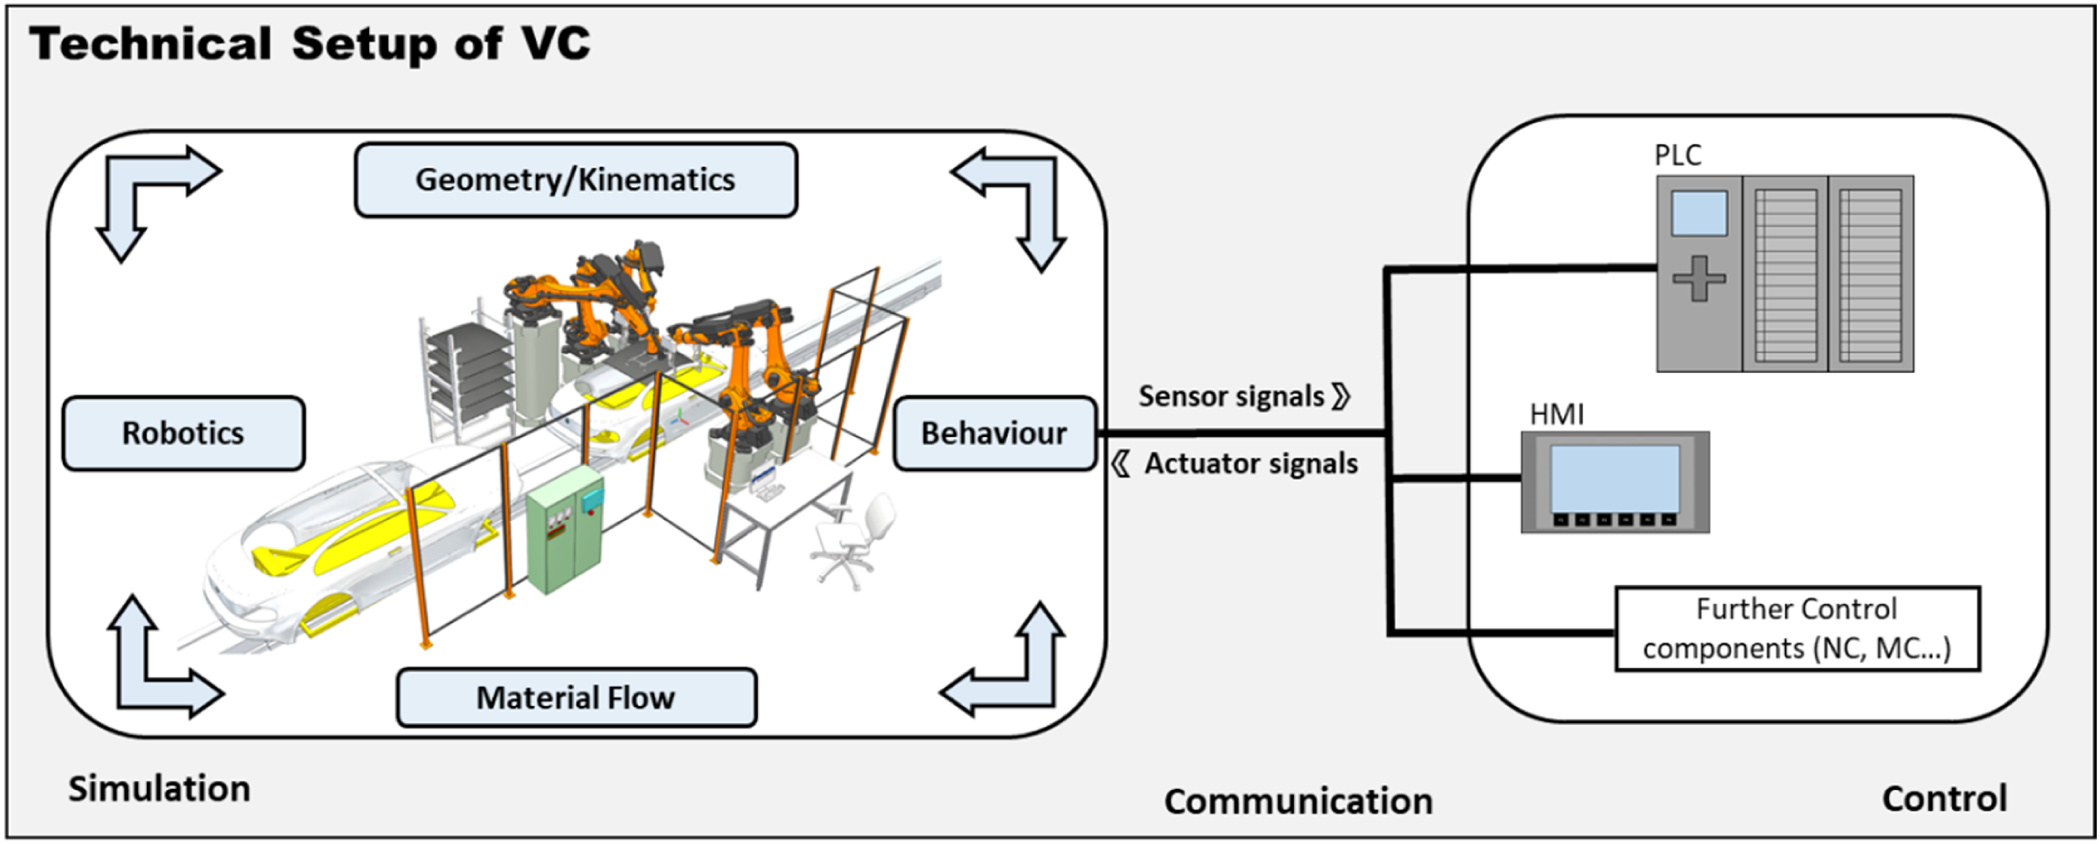
\includegraphics[width=0.92\textwidth]{5-Figures/striffler_vc_technical_configurations.jpeg}
    \caption{Technical configurations of virtual commissioning: Model-in-the-Loop (MiL), Software-in-the-Loop (SiL), and Hardware-in-the-Loop (HiL) \cite{Striffler2023}.}
    \label{fig:striffler_vc_configs}
\end{figure}

When complex multi-body physics equations are needed, game engines can use the \gls{FMI} standard \cite{Chowdhury2025}. External simulation models compiled as \glspl{FMU} compute the physics, while the game engine handles visualization. \textcite{Juhlin2022} showed how combining \glspl{AAS} with \glspl{FMU} allows cloud-based simulation of motor drives.

\subsection{Industrial Communication in the Game Engine Loop}

Connecting a game engine to industrial hardware requires care with thread timing. Game engines run on a continuous loop that updates graphics every frame (often 60 to 120 times per second) and updates physics at fixed intervals (typically 50~Hz, or every 20~ms).

If network queries (\gls{OPCUA}, \gls{MQTT}, or REST) run on the main graphics thread, network delays or packet retransmissions will pause the rendering loop, causing visible stutter \cite{Pajpach2022}.

To avoid this, industrial game engine setups use separate threads \cite{Pajpach2023,Garcia2025}:
\begin{enumerate}
    \item \textbf{Background Threads:} Network communication runs on worker threads that listen for incoming packets without blocking the main loop.
    \item \textbf{Thread-Safe Buffers:} New data values are saved into protected memory buffers.
    \item \textbf{Interpolation:} At each physics tick, the game engine reads the latest values from the buffer. Smooth interpolation (such as Lerp) is used between incoming updates to prevent parts from jumping abruptly when network packets arrive unevenly \cite{Pajpach2022,Pajpach2023}.
\end{enumerate}

\Cref{fig:pajpach_unity_dataflow} shows an example architecture from \textcite{Pajpach2023}, where Unity 3D retrieves 3D models from an \gls{AAS} repository and exchanges runtime signals with a physical PLC through an OPC UA server and Node-RED middleware. Similarly, \textcite{Garcia2025} used Unity 3D with BaSyx AAS data spaces for remote line monitoring.

\begin{figure}[htbp]
    \centering
    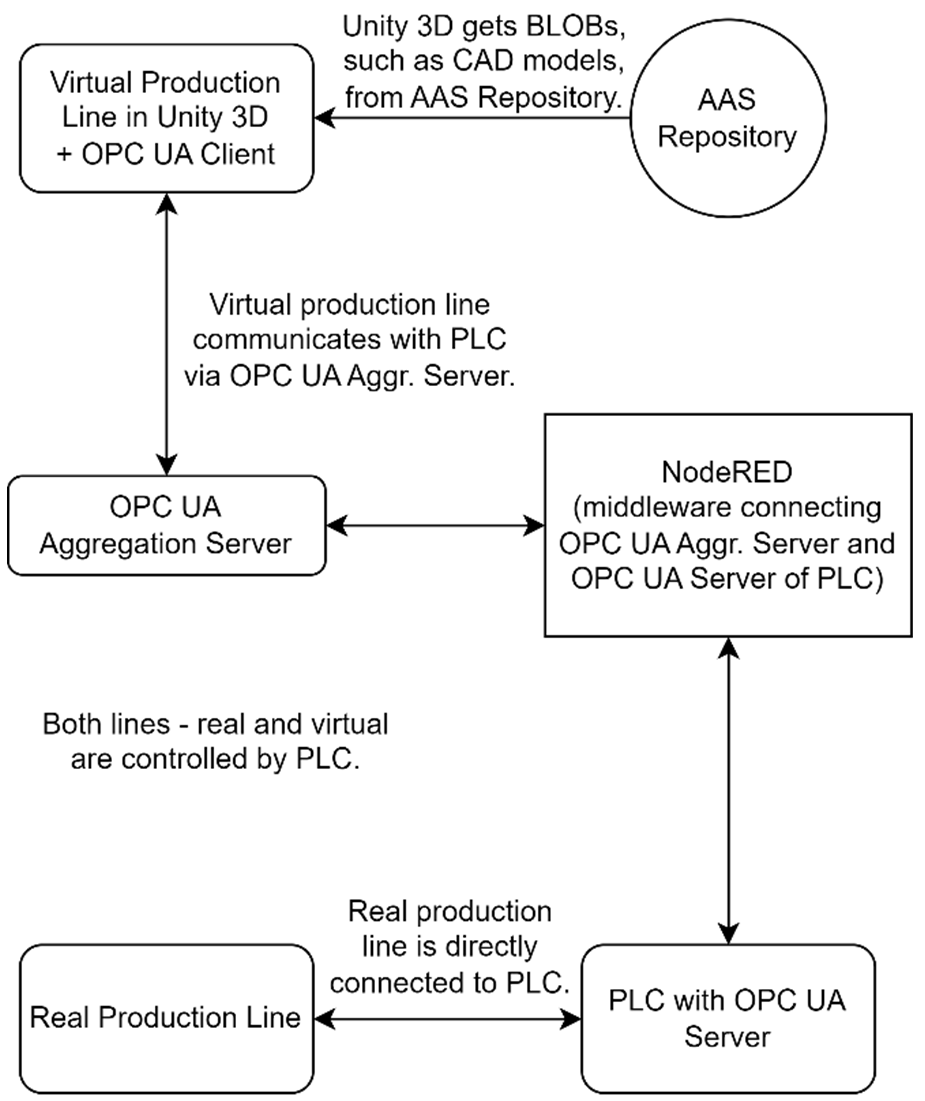
\includegraphics[width=0.72\textwidth]{5-Figures/pajpach_dt_unity_dataflow.png}
    \caption{Architecture and data flow in an educational digital twin using Unity 3D, AAS, and OPC UA \cite{Pajpach2023}.}
    \label{fig:pajpach_unity_dataflow}
\end{figure}

%=============================================================================
\section{Automated Generation of Digital Twins}
\label{sec:automated_dt_generation}
%=============================================================================

While digital twins offer clear benefits, the engineering effort required to build and maintain them remains high, especially for smaller manufacturers \cite{Alexopoulos2025,Schaper2025}.

\subsection{Bottlenecks in Manual Workflows}

Traditional digital twin development is mostly manual. As shown in \Cref{fig:toolchain_fragmentation}, engineering data is split across different tools \cite{Schaper2025}: mechanical engineers work in \gls{CAD}, electrical engineers design schematics in \gls{ECAD}, software developers write PLC code in vendor tools, and asset data is stored in \gls{PLM} or \gls{MES} databases.

\begin{figure}[htbp]
    \centering
    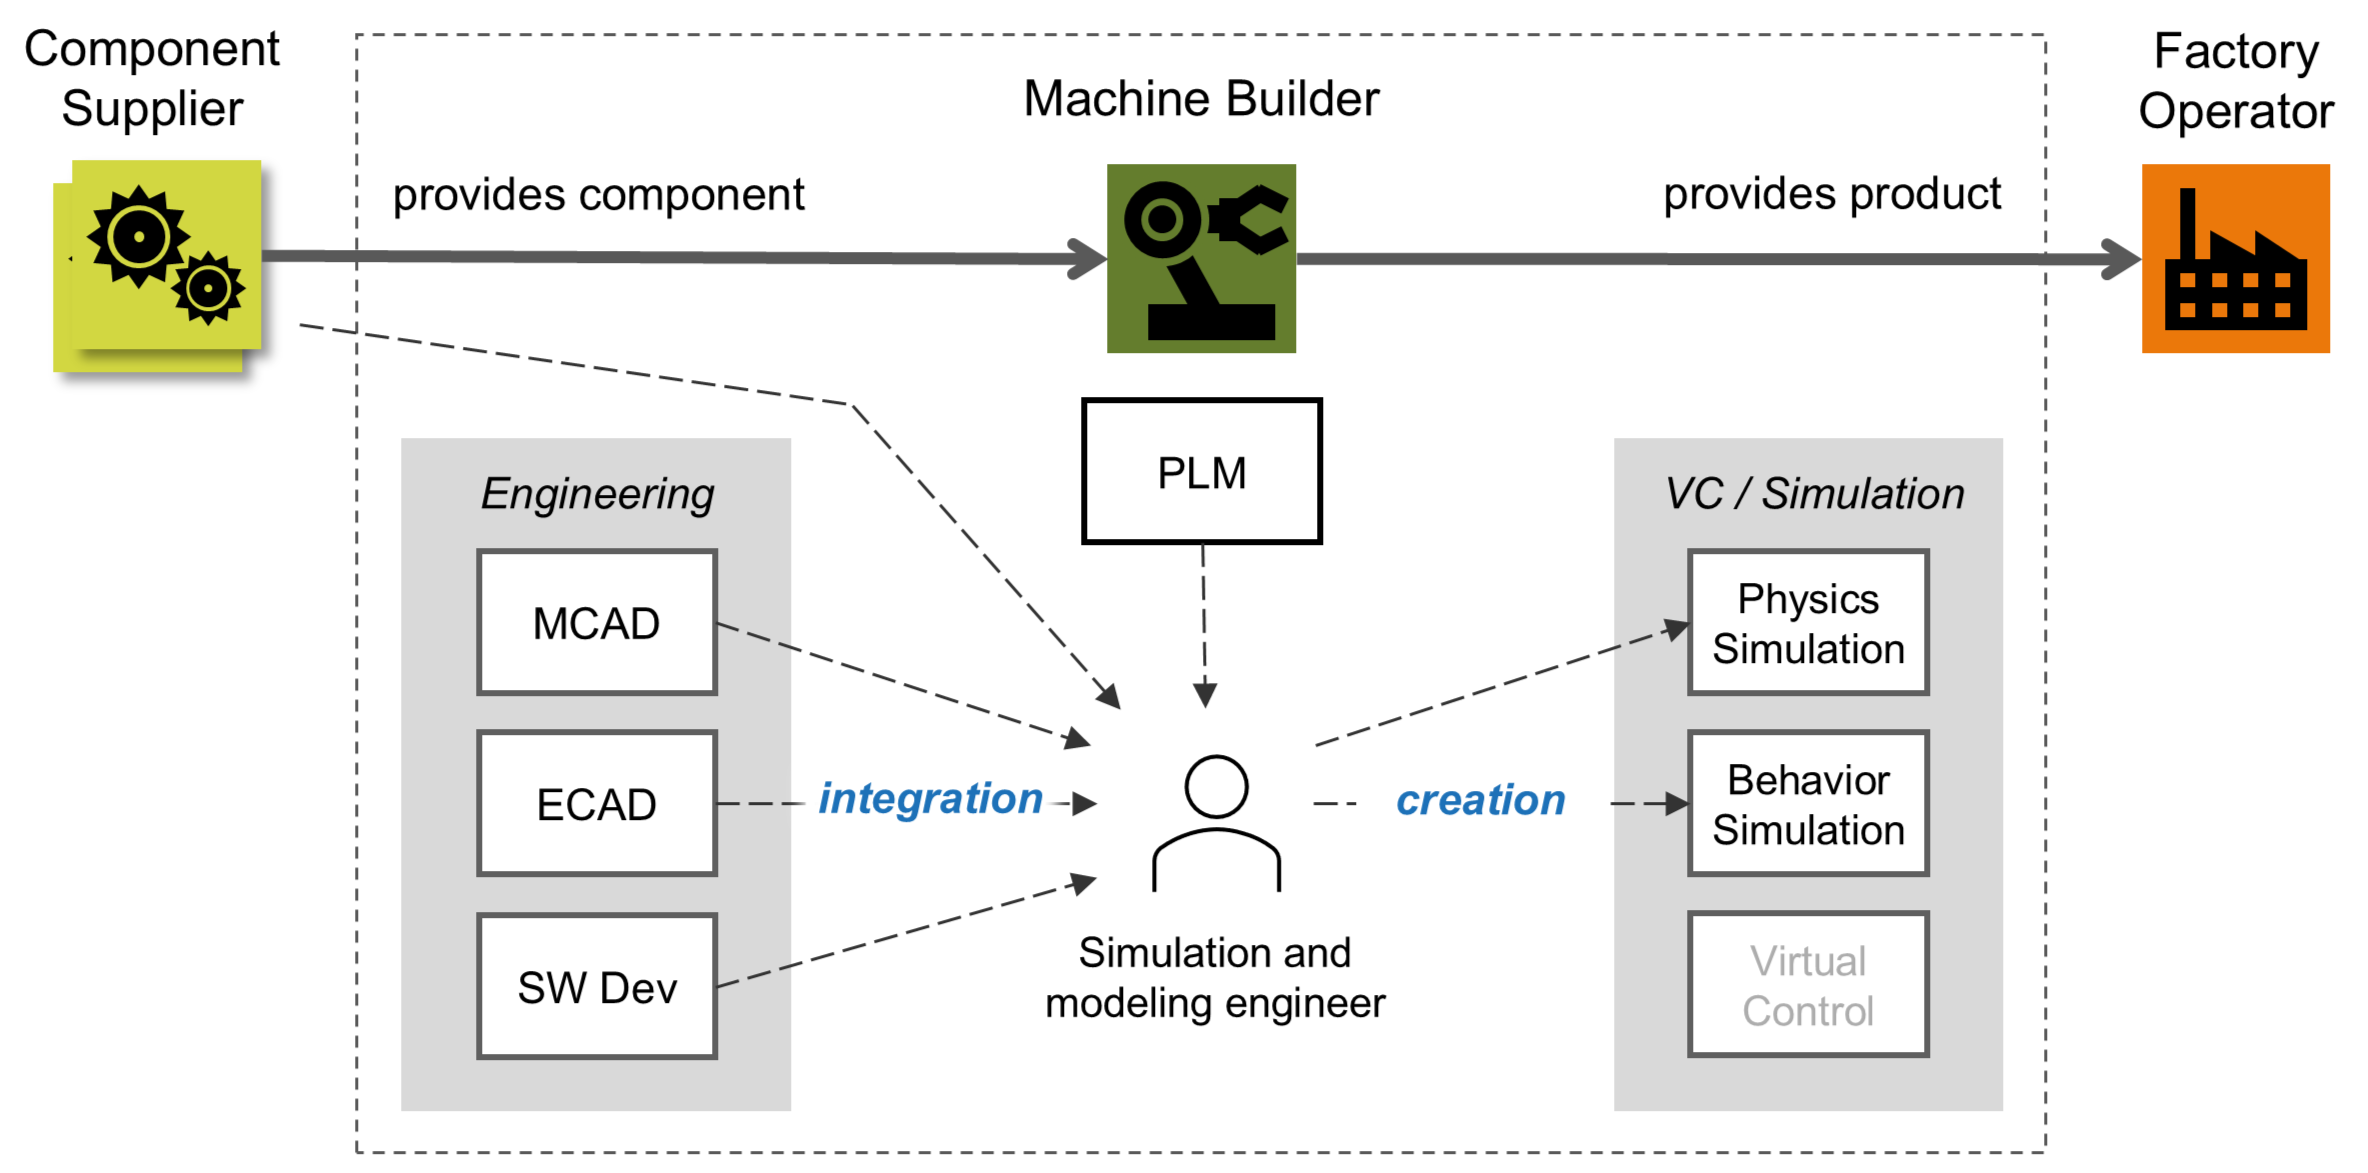
\includegraphics[width=0.88\textwidth]{5-Figures/schaper_toolchain_bottleneck.png}
    \caption{Data fragmentation across engineering tools in machine development \cite{Schaper2025}.}
    \label{fig:toolchain_fragmentation}
\end{figure}

To build a simulation model, an engineer has to collect all these files, import 3D meshes into the engine, set up parent-child relationships, configure joint limits, and manually connect virtual sensors to PLC addresses \cite{Alexopoulos2025,Koch2024}.

This manual approach has three main drawbacks:
\begin{enumerate}
    \item \textbf{High Time and Cost:} Building a model for a single workstation can take several weeks of engineering work \cite{Garcia2023}.
    \item \textbf{Risk of Configuration Errors:} Connecting hundreds of signal addresses by hand easily leads to mistakes that can cause simulation bugs.
    \item \textbf{Maintenance Delays:} In reconfigurable factories, machines are frequently moved or swapped. If the simulation model is not updated immediately, it quickly becomes outdated and unreliable \cite{Ahvanouee2025,Herzog2025}.
\end{enumerate}

To address these issues, recent research focuses on automating digital twin creation. Existing methods generally follow model-driven, data-driven, or AI-based approaches.

\subsection{Model-Driven Approaches}

Model-driven approaches use existing engineering files as the source to build the digital twin components, 3D scenes, and signal connections automatically \cite{Luder2020,Ahvanouee2025}.

Examples include:
\begin{itemize}
    \item \textbf{AutomationML-Based Methods:} \textcite{Alexopoulos2025} parse \gls{AML} files containing plant topology and device types to instantiate 3D machines and set up communication drivers in Unity, as shown in \Cref{fig:alexopoulos_architecture}. \textcite{Chowdhury2025} extract part relationships and mass properties from CAD files to assemble motion models in Unreal Engine using FMI.
    \item \textbf{AAS-Based Configuration:} \textcite{Pretz2025} use \gls{AAS} descriptions to configure autonomous mobile robots (\glspl{AMR}) automatically. \textcite{Ahvanouee2025} use AAS submodels to exchange data between different engineering tools across supply chain partners.
    \item \textbf{SysML Models:} \textcite{Heermann2024} use textual \gls{SysML}~v2 models to generate digital twin software modules and MQTT topic structures.
    \item \textbf{ECAD and Multi-Physics Synthesis:} \textcite{Schaper2025} parse electrical and fluid schematics together with AAS component data to connect FMU simulation blocks automatically. \textcite{Koch2024} similarly generate simulation models using structured component descriptions.
    \item \textbf{Automatic AAS Assembly:} \textcite{Gollner2022} present a method that queries equipment databases to generate populated AAS files automatically. \textcite{Perez2025} generate Eclipse BaSyx DataBridge configs directly from interface submodels.
\end{itemize}

\begin{figure}[htbp]
    \centering
    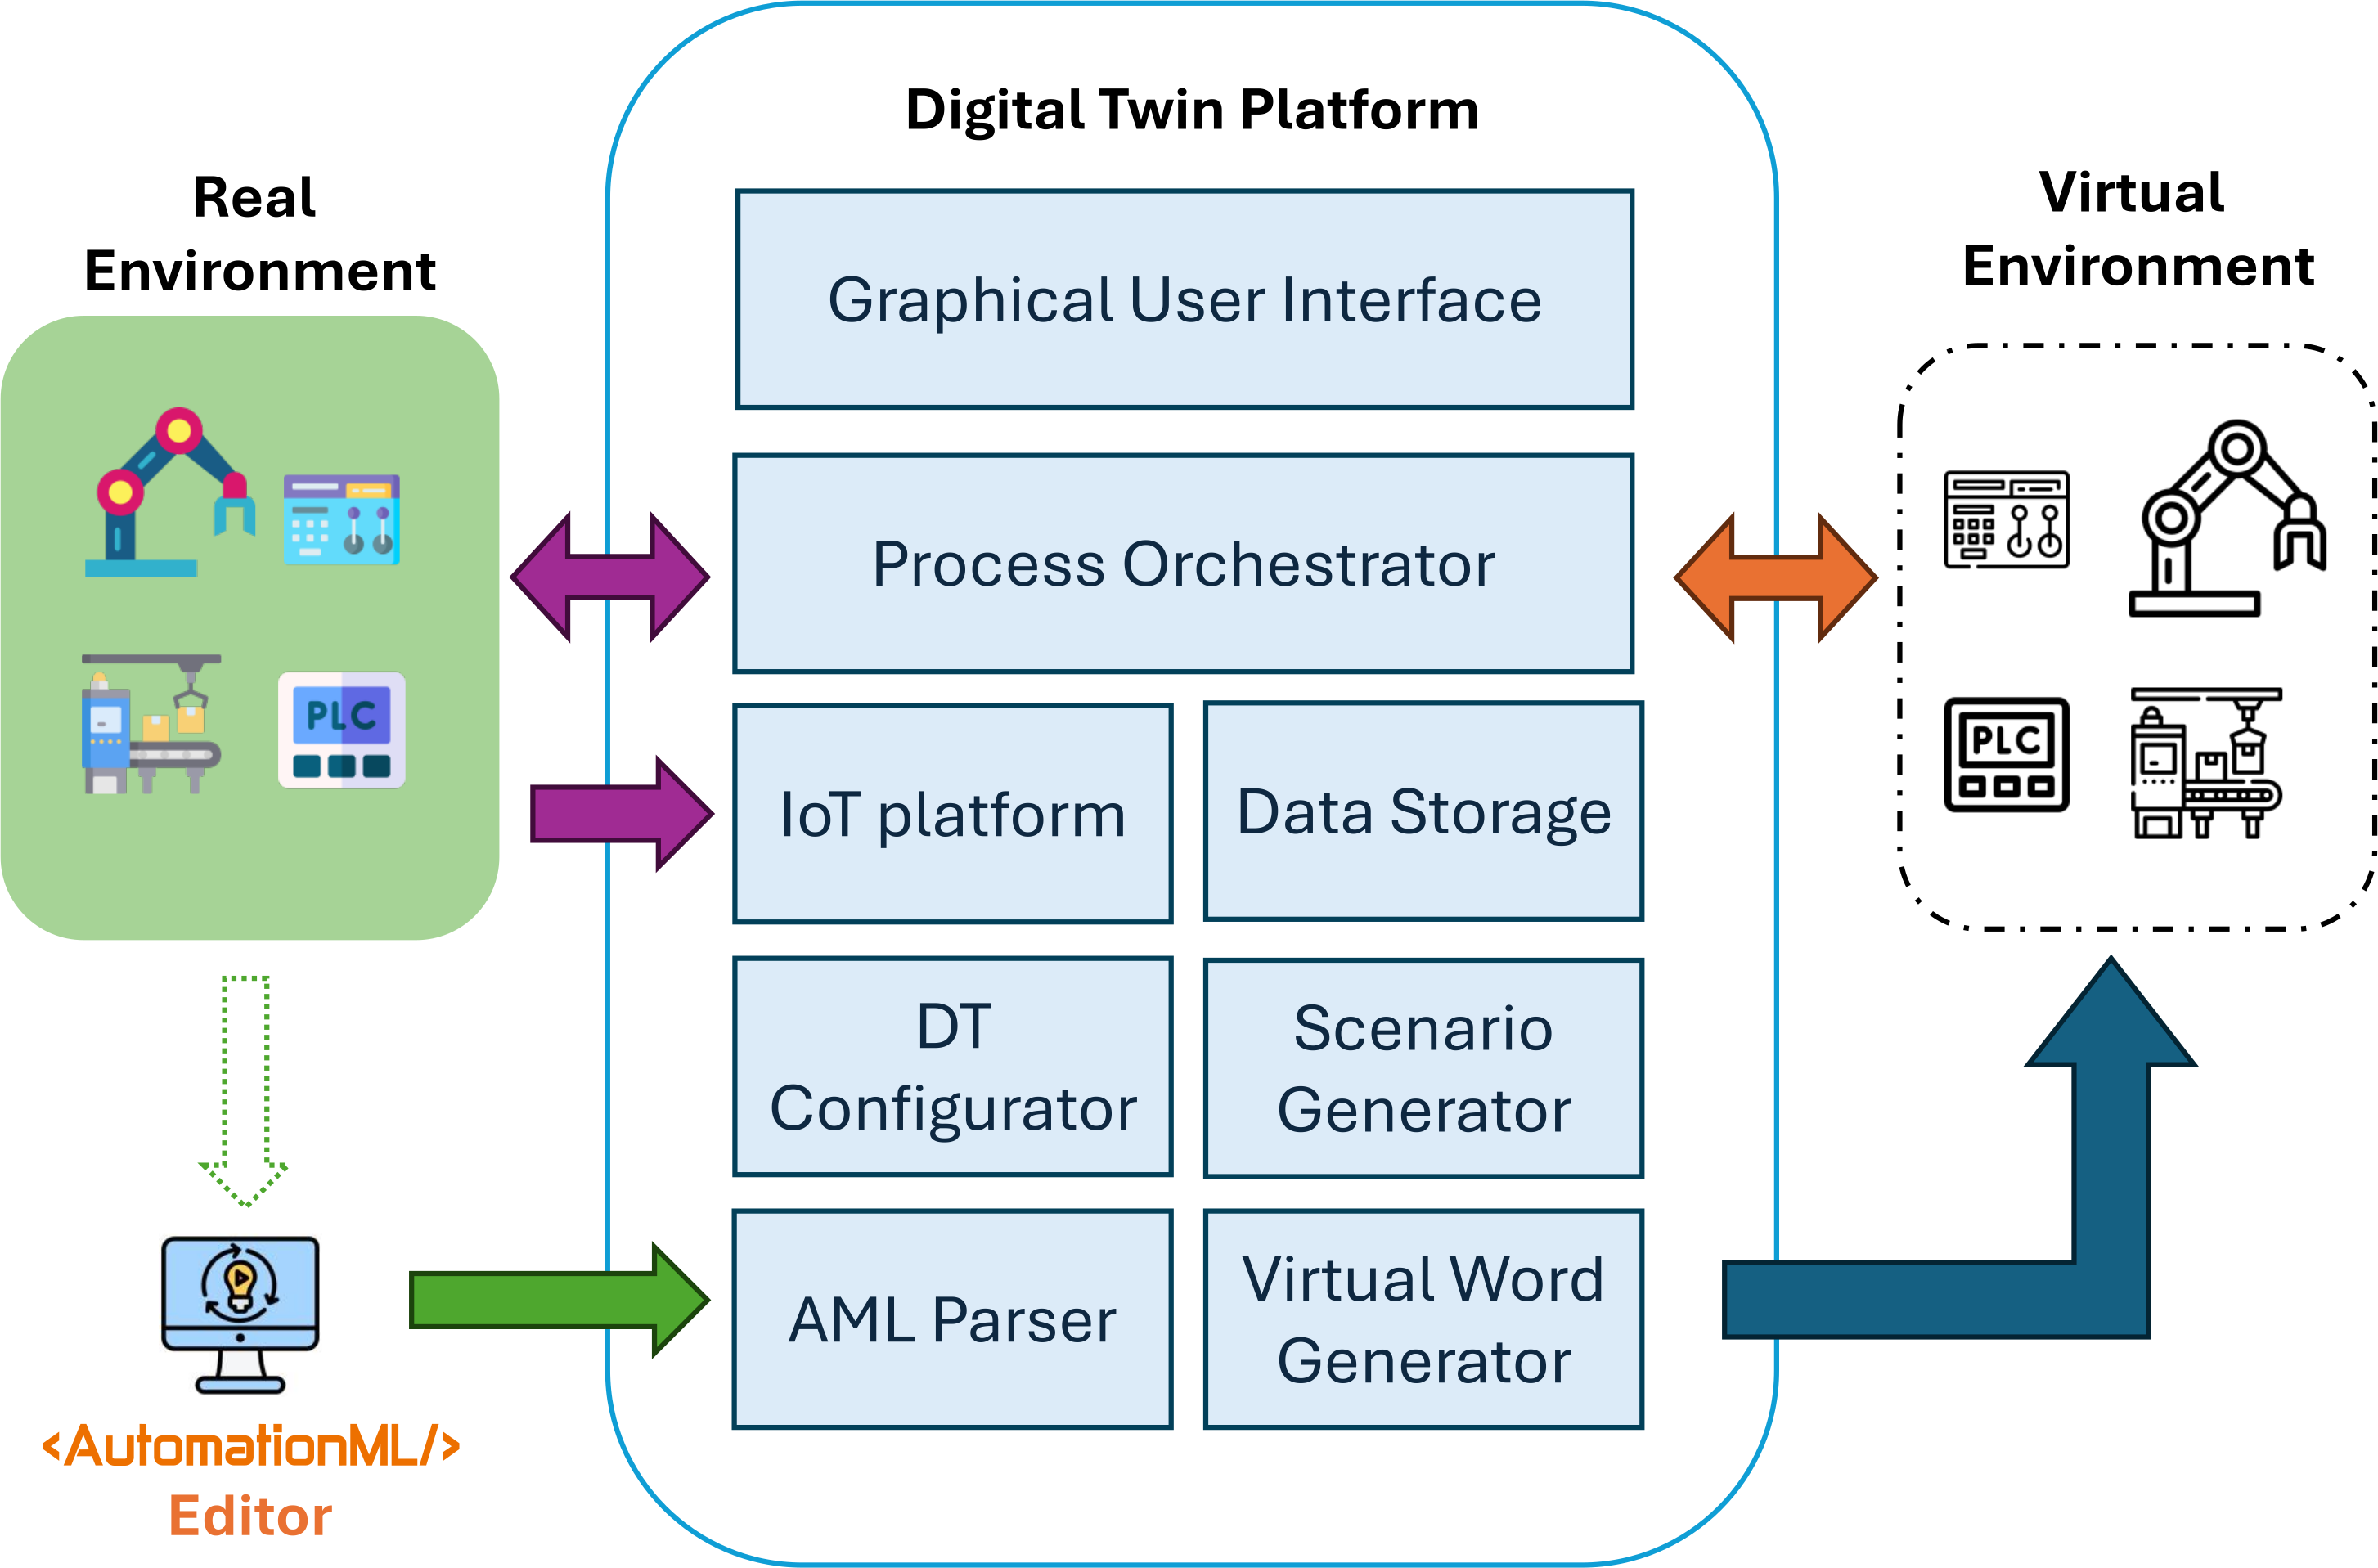
\includegraphics[width=0.88\textwidth]{5-Figures/alexopoulos_dt_architecture.png}
    \caption{Architecture of the model-based platform for automated Digital Twin generation \cite{Alexopoulos2025}.}
    \label{fig:alexopoulos_architecture}
\end{figure}

Model-driven methods provide reliable, deterministic results because they follow validated engineering designs. However, they require clean, up-to-date source files.

\subsection{Data-Driven Approaches}

In older factories where machines lack up-to-date CAD or design files, data-driven methods discover the digital twin structure from historical and live sensor data \cite{Lugaresi2021,Garcia2023}:
\begin{itemize}
    \item \textbf{Process Mining from Event Logs:} \textcite{Lugaresi2021} apply process mining to timestamped machine logs to determine routing, part flows, and buffer queues, building discrete event simulation models without design drawings.
    \item \textbf{Machine Learning Surrogates:} \textcite{Garcia2023} train machine learning models on sensor readings to estimate energy use, creating behavior models directly from measurement data.
\end{itemize}

Data-driven methods work well when engineering files are missing, but they produce approximations rather than exact 3D geometric models and depend heavily on having clean sensor data.

\subsection{Generative AI and Large Language Models}

Recent work explores using \glspl{LLM} and generative AI to assist in creating digital twins \cite{Dong2024,Alexopoulos2025}.

\begin{figure}[htbp]
    \centering
    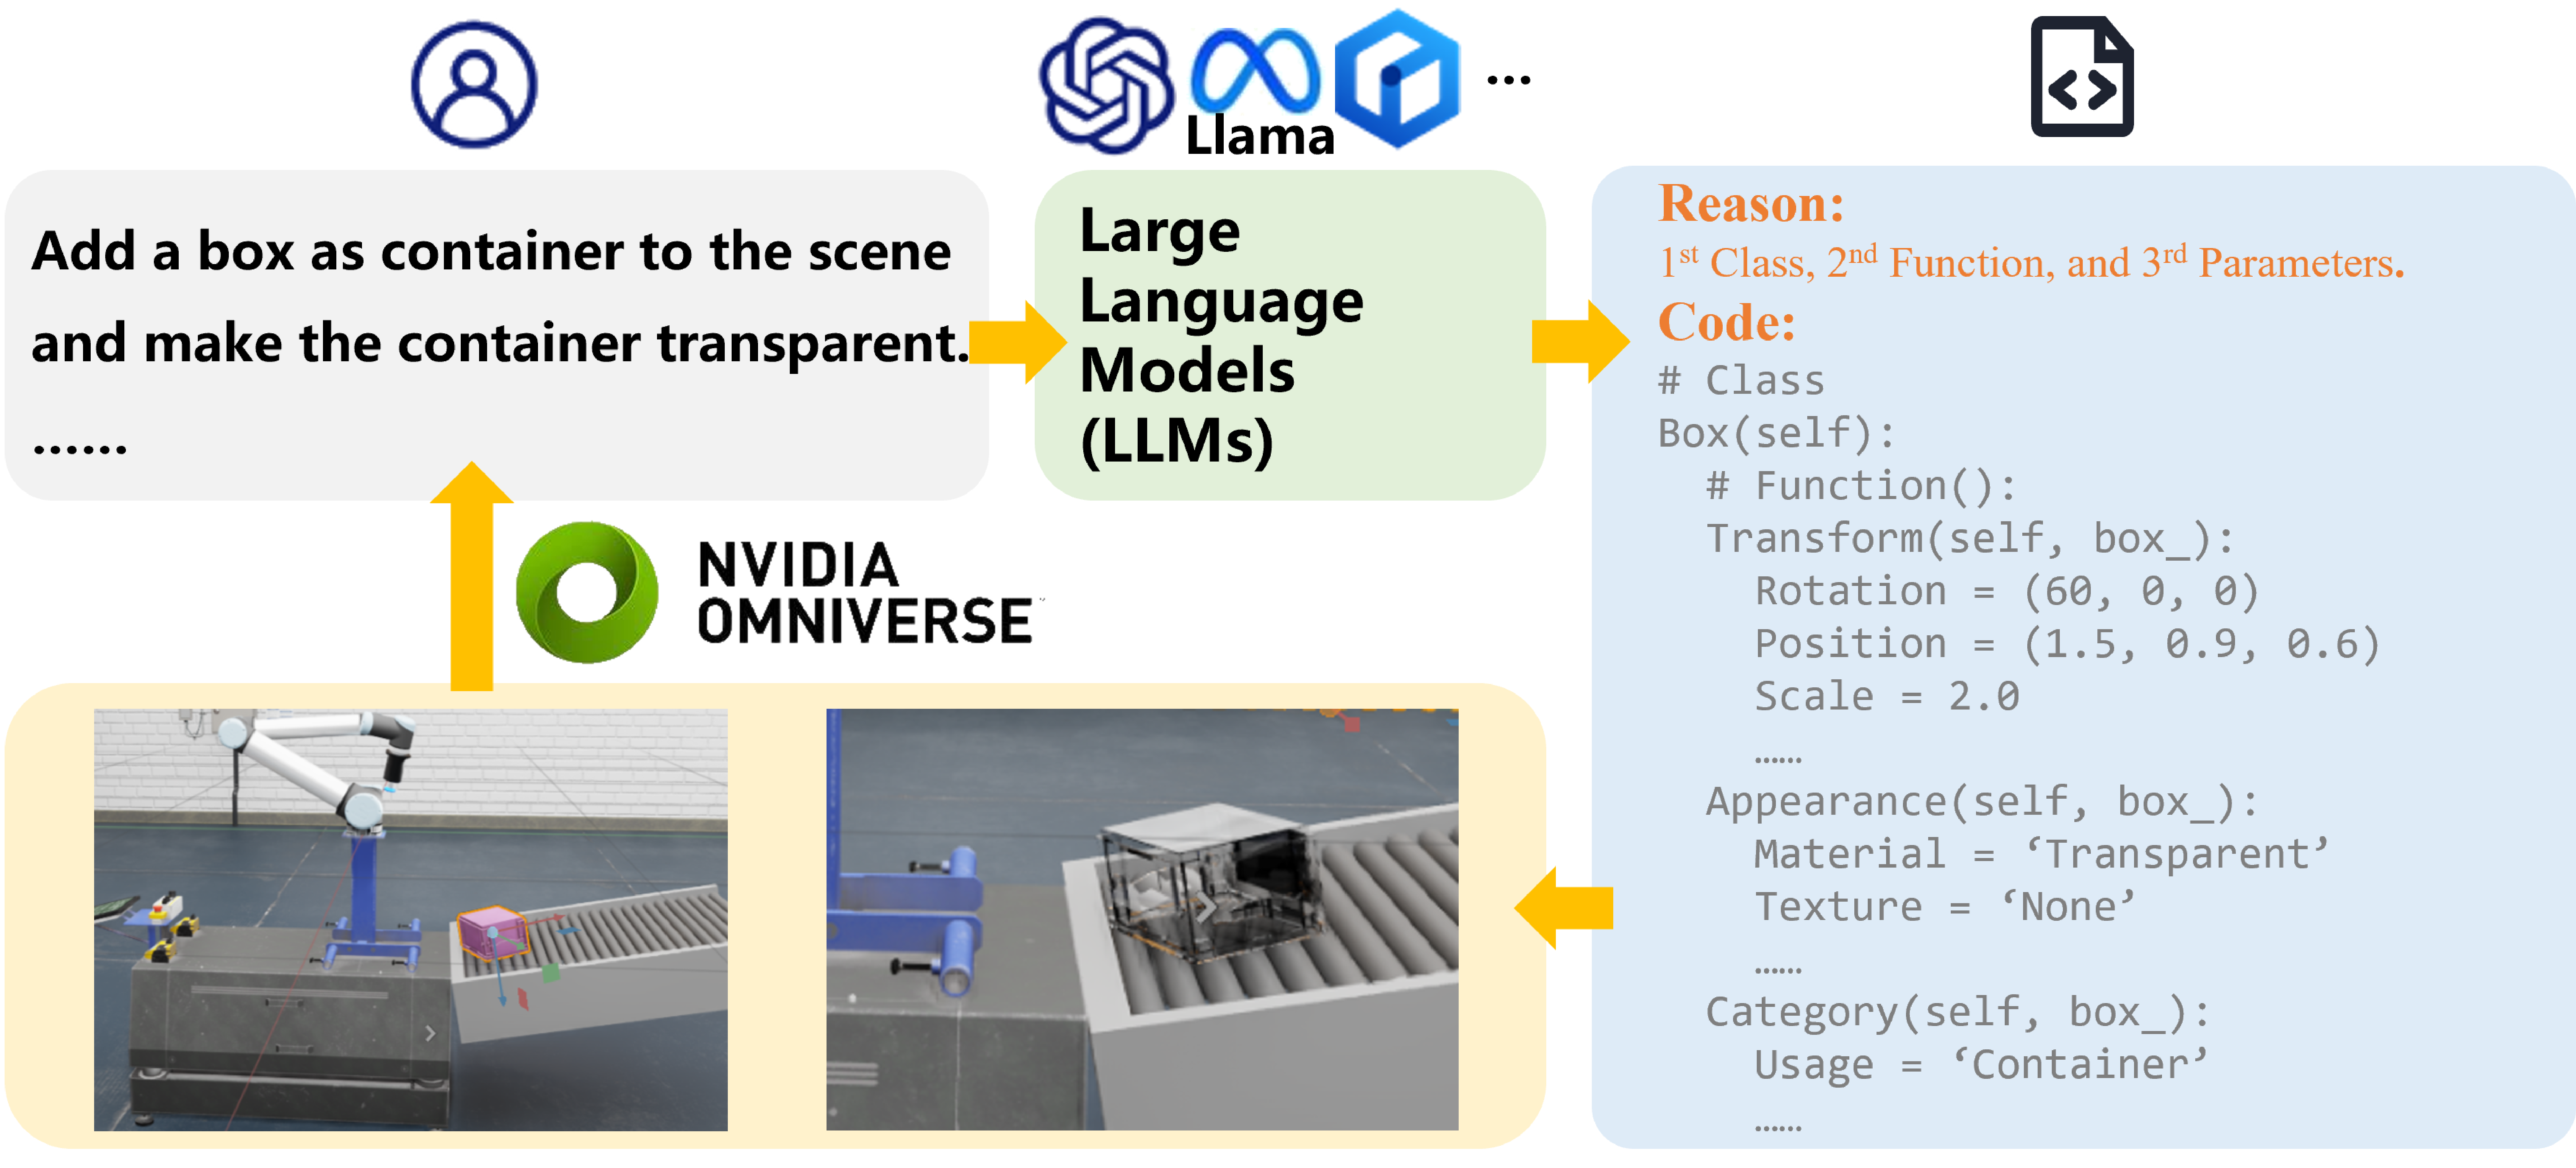
\includegraphics[width=0.88\textwidth]{5-Figures/nvidia_llm.pdf} 
    \caption{Digital twin code generation process for NVIDIA Omniverse using LLMs \cite{Dong2024}.}
    \label{fig:llm_nvidia_omniverse}
\end{figure}

As shown in \Cref{fig:llm_nvidia_omniverse}, \textcite{Dong2024} use an \gls{LLM} that translates natural language prompts into Python scripts that build 3D scenes in NVIDIA Omniverse. \textcite{Alexopoulos2025} use LLMs to generate simulation test scenarios as BPMN process charts.

While LLMs are flexible, their outputs can vary and sometimes contain errors. In industrial automation, deterministic behavior is essential for machine safety, meaning AI tools are better suited as assistants for testing rather than for generating core machine structures.

\subsection{Synthesis of State-of-the-Art Approaches}

Comparing these methods highlights clear trade-offs. Model-driven methods \cite{Alexopoulos2025,Schaper2025} provide reliable structures, but usually end in pre-built scenes that cannot adapt dynamically at runtime. Data-driven methods \cite{Lugaresi2021,Garcia2023} are useful for legacy equipment, but lack detailed 3D geometry and kinematics. Generative AI methods \cite{Dong2024} make initial scene drafting fast, but lack the consistency needed for control systems. Most importantly, nearly all existing solutions still require an engineer to manually assemble 3D assets in the simulation editor before compilation, making rapid reconfiguration on the factory floor difficult.

%=============================================================================
\section{Identified Research Gaps and Opportunities}
\label{sec:sota_gaps}
%=============================================================================

Reviewing the literature shows that while individual pieces of the digital twin puzzle (such as 3D mesh optimization, AAS servers, and game engine visualization) have progressed, integrating them into an automated procedural system remains an open challenge. Four main gaps stand out:

\begin{enumerate}
    \item \textbf{Gap 1: Fragmented Aspects vs. Unified Semantic Metamodel.}
    Most tools focus on only one part of the problem. 3D extraction tools \cite{Chowdhury2025,Dong2024} handle meshes but ignore electrical I/O and control logic. In contrast, semantic tools \cite{Gollner2022,Perez2025} manage data properties but treat 3D graphics as an unrelated external viewer. An open submodel schema is needed that combines 3D meshes, kinematic limits, virtual I/O pins, and control logic rules in a single portable package.
    
    \item \textbf{Gap 2: Proprietary Formats vs. Standardized AAS Source of Truth.}
    Several automated systems generate custom scripts or prefabs tied to a specific simulation tool \cite{Alexopoulos2025,Schaper2025,Koch2024}. Once generated, the digital asset cannot easily share its state with other factory systems. Keeping the standardized \gls{AAS} as the main runtime source of truth ensures the digital twin remains accessible across different tools.
    
    \item \textbf{Gap 3: Pre-Compiled Scenes vs. Runtime Procedural Instantiation.}
    In most game engine setups \cite{Alexopoulos2025,Pajpach2022,Garcia2025}, the 3D scene must be manually built and compiled ahead of time. If a physical machine is added or swapped on the shop floor, the simulation program must be recompiled. A system that can download self-contained \gls{AASX} files from a repository at runtime and assemble meshes, joints, and network links in memory would remove this bottleneck.
    
    \item \textbf{Gap 4: Offline Simulation vs. Live Closed-Loop Synchronization.}
    Virtual commissioning tools \cite{Striffler2023,Schaper2025} work well for offline logic testing, but rarely support continuous online synchronization with physical equipment due to network timing issues. Conversely, IoT monitoring tools display live data but lack physics simulation. A unified framework should support both modes using the same asset description.
\end{enumerate}

To synthesize these gaps, \Cref{tab:sota_comparison} compares the proposed framework against leading approaches in the literature across key architectural capabilities.

\begin{table}[htbp]
    \centering
    \caption{Comparative analysis of state-of-the-art automated Digital Twin frameworks.}
    \label{tab:sota_comparison}
    \renewcommand{\arraystretch}{1.2}
    \resizebox{\textwidth}{!}{%
    \begin{tabular}{lccccc}
        \toprule
        \textbf{Approach} & \textbf{Open Standard} & \textbf{Unified Schema} & \textbf{Procedural} & \textbf{Physics /} & \textbf{Live Hardware} \\
        & \textbf{(AAS / AML)} & \textbf{(3D + I/O + Logic)} & \textbf{Runtime} & \textbf{Colliders} & \textbf{Synchronization} \\
        \midrule
        \textcite{Alexopoulos2025}   & AML            & Partial (CAD + AML)     & No (Pre-compiled) & Yes & No (Simulation only) \\
        \textcite{Schaper2025}       & AAS / AML      & No (FMU focused)        & No (Offline VC)   & Yes & No (Offline SiL) \\
        \textcite{Chowdhury2025}     & Proprietary    & No (Kinematics only)    & Partial (Editor)  & Yes & No (Offline) \\
        \textcite{Perez2025}         & AAS            & No (Signals only)       & No                & No  & Yes (DataBridge) \\
        \textcite{Pajpach2023}       & AAS / OPC UA   & No (Separate models)    & No (Pre-compiled) & Yes & Yes (OPC UA polling) \\
        \midrule
        \textbf{This Dissertation}   & \textbf{AAS (IEC 63278)} & \textbf{Yes (AASX package)} & \textbf{Yes (100\% in-memory)} & \textbf{Yes} & \textbf{Yes (Dual-mode)} \\
        \bottomrule
    \end{tabular}%
    }
\end{table}

These gaps motivate the design and research goals of this dissertation. \Cref{cha:architecture} presents the conceptual architecture designed to address these challenges.